\documentclass[11pt]{article}
\usepackage[margin=1in]{geometry}
%%%%%%%%%%%%%%%%%%%%%%%%%%%%%%%%%%%%%%%%%%%%%%%%%%%%%%%%%%%%%%%%%%%%%%%%%%%%
\usepackage{amsmath,amssymb,amsfonts}
\usepackage{amsthm,latexsym,mathrsfs}
\usepackage{bm,bbm,dsfont}
\usepackage{color,graphicx}
\graphicspath{{../figures/}}
\DeclareGraphicsExtensions{.png,.pdf}
\usepackage[config,labelfont={rm,rm},textfont=rm]{caption,subfig}
\usepackage[latin1]{inputenc}
\usepackage[english]{babel}
\usepackage{xr-hyper}
\usepackage[colorlinks=true,linkcolor=blue,citecolor=blue,urlcolor=blue]{hyperref}
% labels of the main document, prefixed M-: build it first, so that its .aux exists
\externaldocument[M-]{../min_spectral_radius_vaccination}

\theoremstyle{plain}
\newtheorem{theorem}{Theorem}[section]
\newtheorem{lemma}[theorem]{Lemma}
\newtheorem{proposition}[theorem]{Proposition}
\theoremstyle{remark}
\newtheorem{remark}[theorem]{Remark}

\everymath{\displaystyle}
\numberwithin{equation}{section}
\renewcommand{\thesection}{S\arabic{section}}

\title{Supplement: interior penalty method, first and second variation\thanks{Parts of this manuscript were edited with the assistance of an AI tool (Claude Opus 5.5, Anthropic). The authors are solely responsible for all proofs and statements.}}
\author{Zhilan \and John \and Yuliya \and Ludmil}
\date{}

\begin{document}

\maketitle

\begin{abstract}
Supplement to ``Minimizing the spectral radius of a diagonally scaled positive
matrix''. Equation, theorem and section numbers without a prefix S refer to
that document.
\end{abstract}

\section{An interior penalty method for the single dose}\label{sec-barrier}

The minimizer of~\eqref{M-t-program} can be computed by an interior penalty
method: a logarithmic barrier for the constraints~\eqref{M-t-constraint} is
added to the objective function with a weight $\mu>0$, and $\mu$ is driven to
zero; see Fiacco and McCormick~\cite{1968Fiacco_McCormick} and Boyd and
Vandenberghe~\cite[Chapter 11]{2004Boyd_Vandenberghe}.

To introduce the interior point method~\cite[Chapter 11]{2004Boyd_Vandenberghe}, let us now define the interior of the set $\mathcal{K}$ of~\eqref{M-Kt-def} as
$\mathcal{K}^\circ=\left\{\bm t>\mathbbm{1},\ \sum_{p\in I_i}\sigma_{1,p}t_p<c_i,\ i=1:m\right\}$. We introduce a barrier function $B(\bm{t})$ and define a new objective function
$F_\mu(\bm{t})$ as follows:
\begin{equation}\label{psi-hat}
  \begin{aligned}
&F_\mu(\bm{t})=\Psi(\bm{t})+\mu B(\bm{t}), \quad\mbox{for}\quad \mu>0, \quad \mbox{on}\quad \mathcal{K}^\circ, \quad\mbox{where}\\
&B(\bm t)=-\sum_{p=1}^{N}\log\left(t_p-1\right)
-\sum_{i=1}^{m}\log\left(c_i-\sum_{p\in I_i}\sigma_{1,p}t_p\right).
  \end{aligned}
\end{equation}
The next theorem shows that for the
single dose problem this method is well defined for every $\mu>0$, converges to
the minimizer, and gives an explicit bound for the error in the objective
function.
\begin{theorem}\label{barrier}
Let $A_1\ge 0$ be irreducible, and let $\widehat{\bm t}$ be the minimizer
of~\eqref{M-t-program} given by Theorem~\ref{M-global}. Then:
\begin{enumerate}
\renewcommand{\labelenumi}{(\roman{enumi})}
\item For every $\mu>0$ the function $F_\mu$ has a unique minimizer
$\bm t(\mu)$ in $\mathcal{K}^\circ$.
\item For every $\mu>0$,
\begin{equation}\label{gap}
0\le\Psi\left(\bm t(\mu)\right)-\Psi\left(\widehat{\bm t}\right)\le\mu\,m(n+1).
\end{equation}
\item $\bm t(\mu)\to\widehat{\bm t}$ as $\mu\to 0$.
\end{enumerate}
\end{theorem}
\begin{proof}
By Theorem~\ref{M-global} and its proof, $\Psi$ is strictly convex and
continuous on $\{\bm t>0\}$, which contains $\mathcal{K}$.

(i) The set $\mathcal{K}^\circ$ is not empty: it contains the point with
$t_p=1+b_{1i}/\left(2n\,\omega_v\sigma_{1,p}\right)$, $p\in I_i$, for which
$\sum_{p\in I_i}\sigma_{1,p}t_p=c_i-b_{1i}/(2\omega_v)<c_i$.
On $\mathcal{K}^\circ$ each of the $m(n+1)$ affine functions
\begin{equation}\label{slacks}
s_{p}(\bm t)=t_p-1,\qquad
s_{i}(\bm t)=c_i-\sum_{p\in I_i}\sigma_{1,p}t_p
\end{equation}
is positive, so $B$ is finite and, as a sum of the convex functions $-\log s$,
convex. Hence $F_\mu$ is strictly convex on $\mathcal{K}^\circ$ and has at most one
minimizer. On $\mathcal{K}$ every $s$ in~\eqref{slacks} is at most
$C=\max_{i}\max\left(c_i,\max_{p\in I_i}c_i/\sigma_{1,p}\right)$, so each term
$-\log s$ of $B$ is at least $-\log C$ on $\mathcal{K}^\circ$. Fix $\bm t^0\in \mathcal{K}^\circ$,
put $\gamma=F_\mu(\bm t^0)$, and let
$E=\left\{\bm t\in \mathcal{K}^\circ: F_\mu(\bm t)\le \gamma\right\}$.
For $\bm t\in E$ and each $s$ in~\eqref{slacks},
\begin{equation}
-\mu\log s(\bm t)\le\mu B(\bm t)+\mu\left(m(n+1)-1\right)\log C
\le \gamma-\Psi(\widehat{\bm t})+\mu\left(m(n+1)-1\right)\log C,
\end{equation}
so $s(\bm t)\ge\delta=C^{1-m(n+1)}\exp\left(-\left(\gamma-\Psi(\widehat{\bm t})\right)/\mu\right)>0$.
Thus $E$ lies in the compact set
\begin{equation}
\mathcal{K}_\delta=\left\{\bm t\in\mathcal{K}\ :\ s(\bm t)\ge\delta\
\mbox{for every $s$ in~\eqref{slacks}}\right\}\subset \mathcal{K}^\circ,
\end{equation}
on which $F_\mu$ is continuous. As a sublevel set of $F_\mu$ in $\mathcal{K}_\delta$, the
set $E$ is closed, hence compact, and it is not empty since it contains
$\bm t^0$. So $F_\mu$ attains its minimum over $E$, and this is its
minimum over $\mathcal{K}^\circ$.

(ii) The left inequality holds because $\bm t(\mu)\in\mathcal{K}$. Let
$\bm t=\bm t(\mu)$ and, for $p\in I_i$,
\begin{equation}
\lambda_p=\frac{\mu}{t_p-1},\qquad
\nu_i=\frac{\mu}{c_i-\sum_{l\in I_i}\sigma_{1,l}t_l} ,
\end{equation}
so that $\lambda_p>0$, $\nu_i>0$, and the barrier $B$, a sum of logarithms of
affine functions, has the partial derivatives
$\mu\,\partial B/\partial t_p(\bm t)=-\lambda_p+\sigma_{1,p}\nu_i$.
Let $\bm y\in\mathcal{K}$, let $0<s<1$, and put $\bm t_s=\bm t+s(\bm y-\bm t)$.
Since $\bm t\in\mathcal{K}^\circ$, $\bm y\in\mathcal{K}$ and $\mathcal{K}$ is
convex, $\bm t_s\in\mathcal{K}^\circ$, and since $\bm t$ minimizes $F_\mu$
on $\mathcal{K}^\circ$, $F_\mu(\bm t_s)\ge F_\mu(\bm t)$. By convexity,
$\Psi(\bm t_s)\le\Psi(\bm t)+s\left(\Psi(\bm y)-\Psi(\bm t)\right)$, and therefore
\begin{equation}
s\left(\Psi(\bm y)-\Psi(\bm t)\right)+\mu\left(B(\bm t_s)-B(\bm t)\right)\ge 0 .
\end{equation}
We divide by $s$ and let $s\to 0$; the second term tends to
$\mu\sum_p\left(\partial B/\partial t_p\right)(\bm t)\left(y_p-t_p\right)$, and we obtain
\begin{equation}\label{barrier-stationary}
\Psi(\bm y)\ge\Psi(\bm t)
+\sum_{p}\lambda_p\left(y_p-t_p\right)
-\sum_{i}\nu_i\sum_{p\in I_i}\sigma_{1,p}\left(y_p-t_p\right).
\end{equation}
Only the derivatives of $B$ were used, not those of $\Psi$.
In the first sum
$\lambda_p\left(y_p-t_p\right)=\lambda_p\left(y_p-1\right)-\lambda_p\left(t_p-1\right)\ge-\mu$,
so the sum is at least $-mn\mu$. In the second,
\begin{equation}
-\sum_{p\in I_i}\sigma_{1,p}\left(y_p-t_p\right)
=\left(c_i-\sum_{p\in I_i}\sigma_{1,p}y_p\right)-\left(c_i-\sum_{p\in I_i}\sigma_{1,p}t_p\right),
\end{equation}
and $\nu_i\left(c_i-\sum_{p\in I_i}\sigma_{1,p}y_p\right)\ge 0$ while
$\nu_i\left(c_i-\sum_{p\in I_i}\sigma_{1,p}t_p\right)=\mu$, so the second term is at least
$-m\mu$. Hence $\Psi(\bm y)\ge\Psi(\bm t(\mu))-\mu\,m(n+1)$
for every $\bm y\in\mathcal{K}$, and $\bm y=\widehat{\bm t}$ gives~\eqref{gap}.

(iii) Let $\mu_k\to 0$. By~\eqref{gap},
$\Psi\left(\bm t(\mu_k)\right)\to\Psi\left(\widehat{\bm t}\right)$.
The points $\bm t(\mu_k)$ lie in the compact set $\mathcal{K}$; if
$\overline{\bm t}$ is the limit of a subsequence, then by continuity
$\Psi(\overline{\bm t})=\Psi(\widehat{\bm t})$, so
$\overline{\bm t}$ minimizes $\Psi$ on $\mathcal{K}$ and $\overline{\bm t}=\widehat{\bm t}$
by Theorem~\ref{M-global}. Every subsequence of $\left(\bm t(\mu_k)\right)$ thus has a
further subsequence converging to $\widehat{\bm t}$, and therefore
$\bm t(\mu_k)\to\widehat{\bm t}$.
\end{proof}

The method of Theorem~\ref{barrier} minimizes $F_{\mu}$ for a decreasing
sequence of weights $\mu$, each minimization started from the previous
minimizer; by~\eqref{gap} the objective function is within $\mu\,m(n+1)$ of the
minimum, which gives a stopping rule.

\section{First and second variation of the objective function}\label{sec-variation}

Throughout this document $A\ge 0$ is irreducible and $\Phi$ is the
function~\eqref{M-phi-def} of Lemma~\ref{M-log-convex}. For
$\bm\xi\in\mathbb{R}^N$ we write $A_e=A\operatorname{diag}\left(e^{\bm\xi}\right)$
and $\rho=\rho(A_e)$. As in the proof of Lemma~\ref{M-log-convex}, $A_e$ and $A_e^T$
are irreducible, and by Theorem~\ref{M-pf} the spectral radius $\rho>0$ is a
simple eigenvalue and there are $\bm v>0$ and $\bm w>0$ with
\begin{equation}\label{v-perron}
A_e\bm v=\rho\,\bm v,\qquad A_e^T\bm w=\rho\,\bm w,\qquad \langle\bm w,\bm v\rangle=1 .
\end{equation}
We put $\bm\varphi=\bm w\odot\bm v$, so that $\bm\varphi>0$ and
$\sum_p\varphi_p=1$, and $D_w=\operatorname{diag}(\bm w)$,
$D_v=\operatorname{diag}(\bm v)$.

\begin{lemma}\label{v-border}
The matrix
\begin{equation}\label{v-border-matrix}
B=\begin{pmatrix}\rho I-A_e&\bm v\\ \bm w^T&0\end{pmatrix}\in\mathbb{R}^{(N+1)\times(N+1)}
\end{equation}
is nonsingular. For $\bm x\in\mathbb{R}^N$ let $R\bm x=\bm y$, where
$(\bm y,\alpha)$ is the solution of
\begin{equation}\label{v-border-system}
B\begin{pmatrix}\bm y\\ \alpha\end{pmatrix}
=\begin{pmatrix}\bm x-\bm v\langle\bm w,\bm x\rangle\\ 0\end{pmatrix}.
\end{equation}
Then $\alpha=0$, the map $R$ is linear, and
\begin{equation}\label{v-R}
(\rho I-A_e)R=I-\bm v\bm w^T,\qquad R(\rho I-A_e)=I-\bm v\bm w^T,\qquad
R\bm v=0,\qquad \bm w^TR=0 .
\end{equation}
The matrix $R^T$ is obtained in the same way from $A_e^T$, with $\bm v$ and
$\bm w$ exchanged.
\end{lemma}
\begin{proof}
Let $(\rho I-A_e)\bm y+\alpha\bm v=0$ and $\langle\bm w,\bm y\rangle=0$. Pairing
the first equation with $\bm w$ and using $\bm w^T(\rho I-A_e)=0$ gives
$\alpha\langle\bm w,\bm v\rangle=\alpha=0$. Then $(\rho I-A_e)\bm y=0$, and
since $\rho$ is a simple eigenvalue, $\bm y=c\bm v$ with
$c=\langle\bm w,\bm y\rangle=0$. Hence $B$ is nonsingular.

Pairing the first equation of~\eqref{v-border-system} with $\bm w$ gives
$\alpha=\langle\bm w,\bm x\rangle-\langle\bm w,\bm v\rangle\langle\bm w,\bm x\rangle=0$,
so $(\rho I-A_e)R\bm x=\bm x-\bm v\langle\bm w,\bm x\rangle$ and
$\langle\bm w,R\bm x\rangle=0$; these are the first and the last identity
in~\eqref{v-R}, and $R$ is linear since $B^{-1}$ is. For $\bm x=\bm v$ the right-hand side
of~\eqref{v-border-system} vanishes, so $R\bm v=0$. For the second identity let
$\bm x\in\mathbb{R}^N$ and $\bm z=(\rho I-A_e)\bm x$. Then
$\langle\bm w,\bm z\rangle=0$, so $(\rho I-A_e)R\bm z=\bm z=(\rho I-A_e)\bm x$,
hence $R\bm z-\bm x=c\bm v$, and pairing with $\bm w$ gives
$c=-\langle\bm w,\bm x\rangle$. Thus $R(\rho I-A_e)\bm x=\bm x-\bm v\langle\bm w,\bm x\rangle$.

Transposing the second and the third identity in~\eqref{v-R} gives
$(\rho I-A_e^T)R^T=I-\bm w\bm v^T$ and $\bm v^TR^T=0$. The first part of the
proof, applied to the irreducible matrix $A_e^T$ with $\bm v$ and $\bm w$
exchanged, shows that these two identities determine $R^T\bm x$ as the solution of the
corresponding bordered system.
\end{proof}

\begin{theorem}\label{v-phi}
The function $\Phi$ is infinitely differentiable on $\mathbb{R}^N$, and
\begin{equation}\label{v-phi-derivs}
\nabla\Phi(\bm\xi)=\bm\varphi,\qquad
\nabla^2\Phi(\bm\xi)=-\operatorname{diag}(\bm\varphi)+\bm\varphi\bm\varphi^T
+\rho\left(D_wRD_v+D_vR^TD_w\right).
\end{equation}
\end{theorem}
\begin{proof}
Fix $\bm\xi^0$, and let $A_{e,0}$, $\rho_0$, $\bm v$, $\bm w$ and $R$ be the
quantities above at $\bm\xi^0$. The function
$F:\mathbb{R}^N\times\mathbb{R}^N\times\mathbb{R}\to\mathbb{R}^{N+1}$,
\begin{equation}
F(\bm\xi,\bm x,\lambda)=\begin{pmatrix}\left(\lambda I-A\operatorname{diag}\left(e^{\bm\xi}\right)\right)\bm x\\ \langle\bm w,\bm x\rangle-1\end{pmatrix},
\end{equation}
is infinitely differentiable, $F(\bm\xi^0,\bm v,\rho_0)=0$, and its Jacobian
with respect to $(\bm x,\lambda)$ at this point is the matrix $B$
of~\eqref{v-border-matrix} with its first block row multiplied by $-1$, nonsingular by
Lemma~\ref{v-border}. By the implicit function theorem there are a
neighbourhood $U$ of $\bm\xi^0$ and infinitely differentiable functions
$\bm x(\bm\xi)$ and $\lambda(\bm\xi)$ on $U$ with $\bm x(\bm\xi^0)=\bm v$,
$\lambda(\bm\xi^0)=\rho_0$ and
$A\operatorname{diag}\left(e^{\bm\xi}\right)\bm x(\bm\xi)=\lambda(\bm\xi)\bm x(\bm\xi)$.
Since $\bm v>0$ we may take $U$ so small that $\bm x(\bm\xi)>0$ on $U$. For
$\bm\xi\in U$ let $\widetilde{\bm w}>0$ be the vector given by Theorem~\ref{M-pf}
for $\left(A\operatorname{diag}\left(e^{\bm\xi}\right)\right)^T$; then
$\lambda(\bm\xi)\langle\widetilde{\bm w},\bm x(\bm\xi)\rangle
=\rho\left(A\operatorname{diag}\left(e^{\bm\xi}\right)\right)\langle\widetilde{\bm w},\bm x(\bm\xi)\rangle$
and $\langle\widetilde{\bm w},\bm x(\bm\xi)\rangle>0$, so
$\lambda(\bm\xi)=\rho\left(A\operatorname{diag}\left(e^{\bm\xi}\right)\right)>0$.
Hence $\Phi=\log\lambda$ is infinitely differentiable on $U$.

Fix $\bm h\in\mathbb{R}^N$, put $H=\operatorname{diag}(\bm h)$ and
$\bm\xi(s)=\bm\xi^0+s\bm h$, and write $A_e(s)$, $\lambda(s)$ and $\bm x(s)$ for
the quantities at $\bm\xi(s)$, with primes for derivatives in $s$ at $s=0$.
Since $A_e(s)=A_{e,0}\operatorname{diag}\left(e^{s\bm h}\right)$, we have $A_e'=A_{e,0}H$ and
$A_e''=A_{e,0}H^2$. Differentiating $A_e(s)\bm x(s)=\lambda(s)\bm x(s)$ and
$\langle\bm w,\bm x(s)\rangle=1$ once and twice at $s=0$,
\begin{align}
&A_e'\bm v+A_{e,0}\bm x'=\lambda'\bm v+\rho_0\bm x',\qquad \langle\bm w,\bm x'\rangle=0,\label{v-first}\\
&A_e''\bm v+2A_e'\bm x'+A_{e,0}\bm x''=\lambda''\bm v+2\lambda'\bm x'+\rho_0\bm x'' .\label{v-second}
\end{align}
Pairing~\eqref{v-first} with $\bm w$ and using $\bm w^TA_{e,0}=\rho_0\bm w^T$ gives
\begin{equation}
\lambda'=\bm w^TA_{e,0}H\bm v=\rho_0\,\bm w^TH\bm v=\rho_0\langle\bm\varphi,\bm h\rangle,
\end{equation}
so the derivative of $\Phi\left(\bm\xi(s)\right)$ at $s=0$ is
$\lambda'/\rho_0=\langle\bm\varphi,\bm h\rangle$, which is the first identity
in~\eqref{v-phi-derivs}. Moreover~\eqref{v-first} gives
$(\rho_0I-A_{e,0})\bm x'=A_e'\bm v-\lambda'\bm v=\left(I-\bm v\bm w^T\right)A_e'\bm v$,
since $\bm w^TA_e'\bm v=\lambda'$, and with $\langle\bm w,\bm x'\rangle=0$ and
Lemma~\ref{v-border}, $\bm x'=RA_e'\bm v=RA_{e,0}H\bm v$. Pairing~\eqref{v-second}
with $\bm w$ and using $\langle\bm w,\bm x'\rangle=0$,
\begin{equation}
\lambda''=\bm w^TA_e''\bm v+2\,\bm w^TA_e'\bm x'
=\rho_0\sum_p\varphi_ph_p^2+2\rho_0\,\bm w^THRA_{e,0}H\bm v .
\end{equation}
By~\eqref{v-R}, $RA_{e,0}=R(A_{e,0}-\rho_0I)+\rho_0R=-\left(I-\bm v\bm w^T\right)+\rho_0R$, and therefore
\begin{equation}
\bm w^THRA_{e,0}H\bm v=-\sum_p\varphi_ph_p^2+\langle\bm\varphi,\bm h\rangle^2
+\rho_0\,\bm h^TD_wRD_v\bm h .
\end{equation}
The second derivative of $\Phi\left(\bm\xi(s)\right)$ at $s=0$ is
\begin{equation}
\frac{\lambda''}{\rho_0}-\left(\frac{\lambda'}{\rho_0}\right)^2
=-\sum_p\varphi_ph_p^2+\langle\bm\varphi,\bm h\rangle^2+2\rho_0\,\bm h^TD_wRD_v\bm h ,
\end{equation}
and since $\bm h^TD_wRD_v\bm h=\bm h^TD_vR^TD_w\bm h$, this is $\bm h^T\mathcal{H}\bm h$
with $\mathcal{H}$ the symmetric matrix on the right of~\eqref{v-phi-derivs}.
A symmetric matrix is determined by its quadratic form, so
$\nabla^2\Phi(\bm\xi^0)=\mathcal{H}$.
\end{proof}

By~\eqref{v-R}, $\nabla^2\Phi(\bm\xi)\mathbbm{1}=0$, in agreement with
$\Phi(\bm\xi+c\mathbbm{1})=\Phi(\bm\xi)+c$, and by Lemma~\ref{M-log-convex} the
matrix $\nabla^2\Phi(\bm\xi)$ is positive semidefinite.

\begin{lemma}\label{v-g}
For $\chi_1,\chi_2,\chi_3\ge 0$ the function $g$ of~\eqref{M-g-def}, with the
index $p$ omitted, is $g=P/Q$ with
\begin{equation}\label{v-PQ}
\begin{aligned}
P&=\omega_v+(1-\varepsilon_1)\chi_1+\varepsilon_2\chi_2+\frac{\varepsilon_2}{\omega}\chi_1\chi_2,\\
Q&=\omega_v+\chi_1+\varepsilon_2\chi_2+\frac{2\varepsilon_2}{\omega}\chi_1\chi_2
+\frac{\varepsilon_2\varepsilon_3}{\omega^2}\chi_1\chi_2\chi_3 .
\end{aligned}
\end{equation}
In particular $P,Q\ge\omega_v>0$, and $\xi=\log g=\log P-\log Q$ satisfies
\begin{equation}\label{v-logg}
\frac{\partial\xi}{\partial\chi_k}=\frac{\partial_kP}{P}-\frac{\partial_kQ}{Q},\qquad
\frac{\partial^2\xi}{\partial\chi_k\partial\chi_l}
=\frac{\partial_{kl}P}{P}-\frac{\partial_kP\,\partial_lP}{P^2}
-\frac{\partial_{kl}Q}{Q}+\frac{\partial_kQ\,\partial_lQ}{Q^2},
\end{equation}
where
\begin{equation}\label{v-PQ-derivs}
\begin{aligned}
\nabla P&=\left(1-\varepsilon_1+\frac{\varepsilon_2}{\omega}\chi_2,\
\varepsilon_2+\frac{\varepsilon_2}{\omega}\chi_1,\ 0\right),\\
\nabla Q&=\left(1+\frac{2\varepsilon_2}{\omega}\chi_2+\frac{\varepsilon_2\varepsilon_3}{\omega^2}\chi_2\chi_3,\
\varepsilon_2+\frac{2\varepsilon_2}{\omega}\chi_1+\frac{\varepsilon_2\varepsilon_3}{\omega^2}\chi_1\chi_3,\
\frac{\varepsilon_2\varepsilon_3}{\omega^2}\chi_1\chi_2\right),
\end{aligned}
\end{equation}
$\partial_{kk}P=\partial_{kk}Q=0$, $\partial_{13}P=\partial_{23}P=0$, and
$\partial_{12}P=\varepsilon_2/\omega$,
$\partial_{12}Q=2\varepsilon_2/\omega+\varepsilon_2\varepsilon_3\chi_3/\omega^2$,
$\partial_{13}Q=\varepsilon_2\varepsilon_3\chi_2/\omega^2$,
$\partial_{23}Q=\varepsilon_2\varepsilon_3\chi_1/\omega^2$.
\end{lemma}
\begin{proof}
Multiply the numerator and the denominator of~\eqref{M-g-def} by
$\omega_v+\varepsilon_2\chi_2>0$. By~\eqref{M-yz-def},
$\left(\omega_v+\varepsilon_2\chi_2\right)\pi_1=\chi_1$,
$\left(\omega_v+\varepsilon_2\chi_2\right)\pi_1\pi_2=\varepsilon_2\chi_1\chi_2/\omega$ and
$\left(\omega_v+\varepsilon_2\chi_2\right)\pi_1\pi_2\pi_3
=\varepsilon_2\chi_1\chi_2/\omega+\varepsilon_2\varepsilon_3\chi_1\chi_2\chi_3/\omega^2$,
which gives~\eqref{v-PQ}. Every coefficient in~\eqref{v-PQ} is non-negative,
since $0<\varepsilon_1\le 1$, so $P,Q\ge\omega_v$. The remaining formulas are
direct differentiation; $P$ and $Q$ are affine in each $\chi_k$ separately,
so $\partial_{kk}P=\partial_{kk}Q=0$.
\end{proof}

We return to the setting of Section~\ref{M-sec-three}: $b_{k,i}>0$ for all $k$
and $i$, and $A_1\ge 0$ irreducible. For $\bm u\in\mathcal{S}$ let
$\bm\xi(\bm u)=\log\bm g\left(\bm\chi(\bm u)\right)$, so that
$\Theta(\bm u)=\Phi\left(\bm\xi(\bm u)\right)$ with $\Phi$ as
in~\eqref{M-phi-def} for $A=A_1$, and let $\rho$, $\bm v$, $\bm w$,
$\bm\varphi$ and $R$ be the quantities of~\eqref{v-perron}
and Lemma~\ref{v-border} at $\bm\xi(\bm u)$. With
$c_{k,p}=b_{k,i}/\sigma_{k,p}$ for $p\in I_i$, so that
$\chi_{k,p}=c_{k,p}u_{k,p}$ by~\eqref{M-u-of-chihat}, put
\begin{equation}\label{v-a}
a_{k,p}=c_{k,p}\frac{\partial\xi_p}{\partial\chi_{k,p}},\qquad
E_{kl,p}=c_{k,p}c_{l,p}\frac{\partial^2\xi_p}{\partial\chi_{k,p}\partial\chi_{l,p}},
\end{equation}
given by~\eqref{v-logg} at $\left(\chi_{1,p},\chi_{2,p},\chi_{3,p}\right)$.

\begin{theorem}\label{v-theta}
The function $\Theta$ is infinitely differentiable on a neighbourhood of
$\mathcal{S}$, and for $k,l=1,2,3$ and $p,q=1:N$,
\begin{equation}\label{v-theta-derivs}
\frac{\partial\Theta}{\partial u_{k,p}}=\varphi_p\,a_{k,p},\qquad
\frac{\partial^2\Theta}{\partial u_{k,p}\partial u_{l,q}}
=a_{k,p}\left(\nabla^2\Phi\right)_{pq}a_{l,q}+\delta_{pq}\,\varphi_p\,E_{kl,p},
\end{equation}
with $\nabla^2\Phi$ of~\eqref{v-phi-derivs} at $\bm\xi(\bm u)$. In
particular, for $\bm h\in\mathbb{R}^{3N}$ with $\sum_{p\in I_i}h_{k,p}=0$
for all $k$ and $i$, the directions tangent to $\mathcal{S}$, the first and the second
variation of $\Theta$ at $\bm u$ are
\begin{equation}\label{v-variations}
\delta\Theta(\bm u)[\bm h]=\sum_{p=1}^{N}\varphi_p\zeta_p,\qquad
\delta^2\Theta(\bm u)[\bm h]=\bm\zeta^T\nabla^2\Phi\,\bm\zeta
+\sum_{p=1}^{N}\varphi_p\sum_{k,l=1}^{3}E_{kl,p}h_{k,p}h_{l,p},
\end{equation}
where $\zeta_p=\sum_{k=1}^{3}a_{k,p}h_{k,p}$.
\end{theorem}
\begin{proof}
By Lemma~\ref{v-g}, $P$ and $Q$ are positive on the closed orthant
$\chi\ge 0$, hence, being continuous, on an open neighbourhood of it, and there
$\xi_p=\log P_p-\log Q_p$ is infinitely differentiable. The map
$\bm u\mapsto\bm\chi(\bm u)$ is linear, so $\bm\xi(\bm u)$ is infinitely
differentiable on a neighbourhood of $\mathcal{S}$, and so is $\Theta$, by
Theorem~\ref{v-phi}. The component $\xi_p$ depends only on $u_{1,p}$,
$u_{2,p}$ and $u_{3,p}$, with
$\partial\xi_p/\partial u_{k,p}=a_{k,p}$ and
$\partial^2\xi_p/\partial u_{k,p}\partial u_{l,p}=E_{kl,p}$. The chain rule gives
\begin{equation}
\frac{\partial\Theta}{\partial u_{k,p}}=\frac{\partial\Phi}{\partial\xi_p}a_{k,p},\qquad
\frac{\partial^2\Theta}{\partial u_{k,p}\partial u_{l,q}}
=a_{k,p}\frac{\partial^2\Phi}{\partial\xi_p\partial\xi_q}a_{l,q}
+\delta_{pq}\frac{\partial\Phi}{\partial\xi_p}E_{kl,p},
\end{equation}
and Theorem~\ref{v-phi} gives~\eqref{v-theta-derivs}.
Then~\eqref{v-variations} is $\nabla\Theta^T\bm h$ and
$\bm h^T\nabla^2\Theta\,\bm h$.
\end{proof}

The first identity in~\eqref{v-theta-derivs} is~\eqref{t-grad}: the vector
$\bm w$ of~\eqref{M-perron} is a multiple of the one in~\eqref{v-perron}, and
$\operatorname{diag}(\bm g)A_1^T\bm w=\rho\bm w$ gives
$\left(A_1^T\bm w\right)_pv_p/\rho=w_pv_p/g_p$, while
$\partial\xi_p/\partial\chi_{k,p}=\left(\partial g_p/\partial\chi_{k,p}\right)/g_p$.

A product $\nabla^2\Theta\,\bm h$ needs, besides the eigenvectors
$\bm v$ and $\bm w$ used by the gradient, the two vectors
$R\left(\bm v\odot\bm\zeta\right)$ and $R^T\left(\bm w\odot\bm\zeta\right)$,
that is, one solution of the bordered system~\eqref{v-border-system} and one of the
corresponding system for $A_e^T$, both of order $N+1$. No matrix needs to be
formed: the python file \texttt{second\_variation.py} solves the two systems
by GMRES with products by $A_e$ and $A_e^T$. On the weekly instance of
Section~\ref{sec-three-numerics}, at the barycenter of $\mathcal{S}$, where
$\rho=1.9660001326$, and at a random interior point, where
$\rho=2.0749258646$, the gradient~\eqref{v-theta-derivs} agrees with the
gradient~\eqref{t-grad} computed with $\partial g_p/\partial\chi_{k,p}$ by
complex step to $4.3\cdot 10^{-16}$ and $2.2\cdot 10^{-15}$ relative. For three
random tangent directions $\bm h$ at each point, $\nabla^2\Theta\,\bm h$ agrees
with central differences of $\nabla\Theta$ to $3\cdot 10^{-9}$ relative, and
$\delta^2\Theta(\bm u)[\bm h]$ with the second difference of $\Theta$ with step
$10^{-3}$ to $8\cdot 10^{-6}$ relative.

\section{Optimality conditions for three doses}\label{sec-kkt-three}

With multipliers $\lambda_{k,i}$ for the constraints
$\sum_{p\in I_i}\sigma_{k,p}\chi_{k,p}=b_{k,i}$ and $\nu_{k,p}$ for
$\chi_{k,p}\ge 0$ in~\eqref{M-constraints}, the Lagrangian is
\begin{equation}\label{lagrangian-three}
\mathcal{L}(\bm\chi,\bm\lambda,\bm\nu):=\rho\left(A_1\operatorname{diag}\left(\bm g(\bm\chi)\right)\right)
+\sum_{k=1}^3\sum_{i=1}^m\lambda_{k,i}\left(\sum_{p\in I_i}\sigma_{k,p}\chi_{k,p}-b_{k,i}\right)
-\sum_{k=1}^3\sum_{p=1}^N\nu_{k,p}\,\chi_{k,p}.
\end{equation}
The KKT conditions for the Lagrangian are equivalent to (for $k=1:3$, $i=1:m$ and $p\in I_i$):
\begin{equation}\label{kkt-three}
\begin{aligned}
&\sum_{p\in I_i}\sigma_{k,p}\chi_{k,p}=b_{k,i},\qquad \chi_{k,p}\ge 0,\qquad \nu_{k,p}\ge 0,\qquad \nu_{k,p}\,\chi_{k,p}=0,\\
&\lambda_{k,i}=\frac{1}{\sigma_{k,p}}\left(\nu_{k,p}-
\frac{\left(A_1^T\bm w\right)_pv_p}{\langle\bm w,\bm v\rangle}\cdot
\frac{\partial g_p}{\partial\chi_{k,p}}\right),
\end{aligned}
\end{equation}
with $\bm v>0$ and $\bm w>0$ as in~\eqref{M-perron} and $g_p$ as
in~\eqref{M-g-def}.
Every local minimizer of~\eqref{M-the-min} satisfies~\eqref{kkt-three}, since
the constraints are affine; the converse does not hold, and a point
satisfying~\eqref{kkt-three} is a local minimizer if, in addition, the Hessian
of $\mathcal{L}$ with respect to $\bm\chi$ is positive definite on the
directions that preserve the dose constraints and vanish where $\nu_{k,p}>0$.

The constraint terms of~\eqref{lagrangian-three} are affine in $\bm\chi$, so
the Hessian of $\mathcal{L}$ with respect to $\bm\chi$ is the Hessian of
$\bm\chi\mapsto\rho\left(A_1\operatorname{diag}\left(\bm g(\bm\chi)\right)\right)$.
We compute it in three steps: the derivatives of $\rho$ with respect to
$\bm g$, the derivatives of $g_p$ with respect to $\chi_{1,p}$, $\chi_{2,p}$,
$\chi_{3,p}$, and their composition. Throughout, $A_1\ge 0$ is irreducible,
$\bm g>0$, $A_{\bm g}=A_1\operatorname{diag}(\bm g)$, $\rho=\rho(A_{\bm g})$, and $\bm v>0$,
$\bm w>0$ are as in~\eqref{M-perron}, normalized by $\langle\bm w,\bm v\rangle=1$.

\begin{lemma}\label{c-border}
The matrix
\begin{equation}\label{c-border-matrix}
B=\begin{pmatrix}\rho I-A_{\bm g}&\bm v\\ \bm w^T&0\end{pmatrix}\in\mathbb{R}^{(N+1)\times(N+1)}
\end{equation}
is nonsingular. For $\bm x\in\mathbb{R}^N$ let $R\bm x=\bm y$, where $(\bm y,\alpha)$
solves
\begin{equation}\label{c-border-system}
B\begin{pmatrix}\bm y\\ \alpha\end{pmatrix}
=\begin{pmatrix}\bm x-\bm v\langle\bm w,\bm x\rangle\\ 0\end{pmatrix}.
\end{equation}
Then $\alpha=0$, $R$ is linear, and
\begin{equation}\label{c-R}
(\rho I-A_{\bm g})R=I-\bm v\bm w^T,\qquad \bm w^TR=0 .
\end{equation}
\end{lemma}
\begin{proof}
Let $(\rho I-A_{\bm g})\bm y+\alpha\bm v=0$ and $\langle\bm w,\bm y\rangle=0$. Pairing
the first equation with $\bm w$ and using $\bm w^T(\rho I-A_{\bm g})=0$ gives
$\alpha\langle\bm w,\bm v\rangle=\alpha=0$. Then $(\rho I-A_{\bm g})\bm y=0$, and since
$\rho$ is a simple eigenvalue (Theorem~\ref{M-pf}), $\bm y=c\bm v$ with
$c=\langle\bm w,\bm y\rangle=0$. Hence $B$ is nonsingular. Pairing the first
equation of~\eqref{c-border-system} with $\bm w$ gives
$\alpha=\langle\bm w,\bm x\rangle-\langle\bm w,\bm v\rangle\langle\bm w,\bm x\rangle=0$,
so $(\rho I-A_{\bm g})R\bm x=\bm x-\bm v\langle\bm w,\bm x\rangle$ and
$\langle\bm w,R\bm x\rangle=0$, which is~\eqref{c-R}; $R$ is linear since
$B^{-1}$ is.
\end{proof}

\begin{lemma}\label{c-rho-g}
The function $\bm g\mapsto\rho\left(A_1\operatorname{diag}(\bm g)\right)$ is
infinitely differentiable on $\{\bm g>0\}$, and
\begin{equation}\label{c-rho-g-derivs}
\frac{\partial\rho}{\partial g_p}=a_p:=\left(A_1^T\bm w\right)_pv_p,\qquad
\nabla^2_{\bm g}\rho=K+K^T,\qquad
K=\operatorname{diag}\left(A_1^T\bm w\right)R\,A_1\operatorname{diag}(\bm v).
\end{equation}
\end{lemma}
\begin{proof}
Fix $\bm g^0>0$, with $A_{\bm g^0}$, $\rho_0$, $\bm v$, $\bm w$ and $R$ at $\bm g^0$.
The function
\begin{equation*}
F(\bm g,\bm x,\lambda)=\begin{pmatrix}\left(\lambda I-A_1\operatorname{diag}(\bm g)\right)\bm x\\
\langle\bm w,\bm x\rangle-1\end{pmatrix}
\end{equation*}
is a polynomial, $F(\bm g^0,\bm v,\rho_0)=0$, and its Jacobian with respect
to $(\bm x,\lambda)$ at this point is $B$ of~\eqref{c-border-matrix} with
its first block row multiplied by $-1$, nonsingular by Lemma~\ref{c-border}.
By the implicit function theorem there are a neighbourhood $U$ of $\bm g^0$
and infinitely differentiable $\bm x(\bm g)$, $\lambda(\bm g)$ on $U$ with
$\bm x(\bm g^0)=\bm v$, $\lambda(\bm g^0)=\rho_0$ and
$A_1\operatorname{diag}(\bm g)\bm x(\bm g)=\lambda(\bm g)\bm x(\bm g)$. Taking
$U$ smaller, $\bm x(\bm g)>0$ on $U$; pairing with the positive left Perron
vector of $A_1\operatorname{diag}(\bm g)$ shows
$\lambda(\bm g)=\rho\left(A_1\operatorname{diag}(\bm g)\right)$ on $U$.

Fix $\bm h\in\mathbb{R}^N$, put $\bm g(s)=\bm g^0+s\bm h$, and write primes
for derivatives in $s$ at $s=0$. Since $A_{\bm g(s)}=A_{\bm g^0}+sA_1\operatorname{diag}(\bm h)$,
$A_{\bm g}'=A_1\operatorname{diag}(\bm h)$ and $A_{\bm g}''=0$. Differentiating
$A_{\bm g(s)}\bm x(s)=\lambda(s)\bm x(s)$ and $\langle\bm w,\bm x(s)\rangle=1$ once and
twice,
\begin{align*}
&A_{\bm g}'\bm v+A_{\bm g^0}\bm x'=\lambda'\bm v+\rho_0\bm x',\qquad \langle\bm w,\bm x'\rangle=0,\\
&2A_{\bm g}'\bm x'+A_{\bm g^0}\bm x''=\lambda''\bm v+2\lambda'\bm x'+\rho_0\bm x'',\qquad
\langle\bm w,\bm x''\rangle=0 .
\end{align*}
Pairing the first line with $\bm w$ gives
$\lambda'=\bm w^TA_1\operatorname{diag}(\bm h)\bm v=\sum_p\left(A_1^T\bm w\right)_pv_ph_p$,
which is the first identity in~\eqref{c-rho-g-derivs}. The first line also
gives $(\rho_0I-A_{\bm g^0})\bm x'=\left(I-\bm v\bm w^T\right)A_{\bm g}'\bm v$ with
$\langle\bm w,\bm x'\rangle=0$, so $\bm x'=RA_{\bm g}'\bm v$ by Lemma~\ref{c-border}
(the solution of~\eqref{c-border-system} is unique). Pairing the second line
with $\bm w$ and using $\langle\bm w,\bm x'\rangle=0$,
\begin{equation*}
\lambda''=2\,\bm w^TA_{\bm g}'\bm x'=2\,\bm w^TA_1\operatorname{diag}(\bm h)\,R\,A_1\operatorname{diag}(\bm h)\bm v
=2\,\bm h^TK\bm h=\bm h^T\left(K+K^T\right)\bm h .
\end{equation*}
A symmetric matrix is determined by its quadratic form, so
$\nabla^2_{\bm g}\rho=K+K^T$.
\end{proof}

\begin{lemma}\label{c-g}
For $\chi_1,\chi_2,\chi_3\ge 0$ the function $g$ of~\eqref{M-g-def}, with the
index $p$ omitted, is $g=P/Q$ with
\begin{equation}\label{c-PQ}
\begin{aligned}
P&=\omega_v+(1-\varepsilon_1)\chi_1+\varepsilon_2\chi_2+\frac{\varepsilon_2}{\omega}\chi_1\chi_2,\\
Q&=\omega_v+\chi_1+\varepsilon_2\chi_2+\frac{2\varepsilon_2}{\omega}\chi_1\chi_2
+\frac{\varepsilon_2\varepsilon_3}{\omega^2}\chi_1\chi_2\chi_3 ,
\end{aligned}
\end{equation}
$P,Q\ge\omega_v>0$, and, with $\partial_k=\partial/\partial\chi_k$,
\begin{equation}\label{c-g-derivs}
\partial_kg=\frac{\partial_kP}{Q}-\frac{P\,\partial_kQ}{Q^2},\qquad
\partial_{kl}g=\frac{\partial_{kl}P}{Q}
-\frac{\partial_kP\,\partial_lQ+\partial_lP\,\partial_kQ+P\,\partial_{kl}Q}{Q^2}
+\frac{2P\,\partial_kQ\,\partial_lQ}{Q^3},
\end{equation}
where
\begin{equation}\label{c-PQ-derivs}
\begin{aligned}
\nabla P&=\left(1-\varepsilon_1+\frac{\varepsilon_2}{\omega}\chi_2,\
\varepsilon_2+\frac{\varepsilon_2}{\omega}\chi_1,\ 0\right),\\
\nabla Q&=\left(1+\frac{2\varepsilon_2}{\omega}\chi_2+\frac{\varepsilon_2\varepsilon_3}{\omega^2}\chi_2\chi_3,\
\varepsilon_2+\frac{2\varepsilon_2}{\omega}\chi_1+\frac{\varepsilon_2\varepsilon_3}{\omega^2}\chi_1\chi_3,\
\frac{\varepsilon_2\varepsilon_3}{\omega^2}\chi_1\chi_2\right),
\end{aligned}
\end{equation}
$\partial_{kk}P=\partial_{kk}Q=0$, $\partial_{13}P=\partial_{23}P=0$,
$\partial_{12}P=\varepsilon_2/\omega$,
$\partial_{12}Q=2\varepsilon_2/\omega+\varepsilon_2\varepsilon_3\chi_3/\omega^2$,
$\partial_{13}Q=\varepsilon_2\varepsilon_3\chi_2/\omega^2$ and
$\partial_{23}Q=\varepsilon_2\varepsilon_3\chi_1/\omega^2$.
\end{lemma}
\begin{proof}
Multiply the numerator and the denominator of~\eqref{M-g-def} by
$\omega_v+\varepsilon_2\chi_2>0$. By~\eqref{M-yz-def},
\begin{align*}
&\left(\omega_v+\varepsilon_2\chi_2\right)\pi_1=\chi_1,\qquad
\left(\omega_v+\varepsilon_2\chi_2\right)\pi_1\pi_2=\frac{\varepsilon_2}{\omega}\chi_1\chi_2,\\
&\left(\omega_v+\varepsilon_2\chi_2\right)\pi_1\pi_2\pi_3
=\frac{\varepsilon_2}{\omega}\chi_1\chi_2+\frac{\varepsilon_2\varepsilon_3}{\omega^2}\chi_1\chi_2\chi_3,
\end{align*}
which gives~\eqref{c-PQ}. All coefficients in~\eqref{c-PQ} are non-negative,
since $0<\varepsilon_1\le 1$, so $P,Q\ge\omega_v$. The formulas~\eqref{c-g-derivs}
are the quotient rule applied twice, and~\eqref{c-PQ-derivs} and the second
derivatives of $P$ and $Q$ are direct differentiation; $P$ and $Q$ are affine
in each $\chi_k$ separately, so $\partial_{kk}P=\partial_{kk}Q=0$.
\end{proof}

\begin{theorem}\label{c-hessian}
The function
$\bm\chi\mapsto\rho\left(A_1\operatorname{diag}\left(\bm g(\bm\chi)\right)\right)$
is infinitely differentiable on a neighbourhood of $\{\bm\chi\ge 0\}$, and for
$k,l=1,2,3$ and $p,q=1:N$,
\begin{equation}\label{c-hessian-formula}
\frac{\partial^2\mathcal{L}}{\partial\chi_{k,p}\,\partial\chi_{l,q}}
=\frac{\partial g_p}{\partial\chi_{k,p}}\left(K+K^T\right)_{pq}
\frac{\partial g_q}{\partial\chi_{l,q}}
+\delta_{pq}\,a_p\,\frac{\partial^2g_p}{\partial\chi_{k,p}\,\partial\chi_{l,p}},
\end{equation}
with $a_p$ and $K$ of~\eqref{c-rho-g-derivs} and the derivatives of $g_p$
of~\eqref{c-g-derivs} at $\left(\chi_{1,p},\chi_{2,p},\chi_{3,p}\right)$.
For $\bm h\in\mathbb{R}^{3N}$ put
$\zeta_p=\sum_{k=1}^3\left(\partial g_p/\partial\chi_{k,p}\right)h_{k,p}$; then
\begin{equation}\label{c-second-variation}
\bm h^T\nabla^2_{\bm\chi}\mathcal{L}\,\bm h
=2\,\bm\zeta^TK\bm\zeta
+\sum_{p=1}^Na_p\sum_{k,l=1}^3\frac{\partial^2g_p}{\partial\chi_{k,p}\,\partial\chi_{l,p}}h_{k,p}h_{l,p}.
\end{equation}
\end{theorem}
\begin{proof}
By Lemma~\ref{c-g}, $P_p$ and $Q_p$ are positive on $\{\bm\chi\ge 0\}$, hence
on a neighbourhood of it, where $g_p=P_p/Q_p$ is infinitely differentiable
and positive. By Lemma~\ref{c-rho-g} the composition is infinitely
differentiable there. Since $g_p$ depends only on $\chi_{1,p}$,
$\chi_{2,p}$ and $\chi_{3,p}$, the chain rule gives
\begin{equation*}
\frac{\partial^2\rho}{\partial\chi_{k,p}\,\partial\chi_{l,q}}
=\frac{\partial g_p}{\partial\chi_{k,p}}\,\frac{\partial^2\rho}{\partial g_p\,\partial g_q}\,
\frac{\partial g_q}{\partial\chi_{l,q}}
+\delta_{pq}\,\frac{\partial\rho}{\partial g_p}\,
\frac{\partial^2g_p}{\partial\chi_{k,p}\,\partial\chi_{l,p}},
\end{equation*}
and Lemma~\ref{c-rho-g} gives~\eqref{c-hessian-formula}, since the
constraint terms of $\mathcal{L}$ are affine.
Then~\eqref{c-second-variation} follows from
$\bm\zeta^T\left(K+K^T\right)\bm\zeta=2\,\bm\zeta^TK\bm\zeta$.
\end{proof}

In matrix form,~\eqref{c-hessian-formula} is
\begin{equation}\label{c-hessian-matrix}
\nabla^2_{\bm\chi}\mathcal{L}=J^T\left(K+K^T\right)J+E,
\end{equation}
where $J\in\mathbb{R}^{N\times 3N}$ and $E\in\mathbb{R}^{3N\times 3N}$ have the
entries
\begin{equation*}
J_{q,(k,p)}=\delta_{pq}\,\frac{\partial g_p}{\partial\chi_{k,p}},\qquad
E_{(k,p),(l,q)}=\delta_{pq}\,a_p\,\frac{\partial^2g_p}{\partial\chi_{k,p}\,\partial\chi_{l,p}};
\end{equation*}
$J$ has three nonzero entries in each row, and $E$ is block diagonal with one
$3\times 3$ block for each $p$. In this notation $\bm\zeta=J\bm h$
in~\eqref{c-second-variation}.

A product $\nabla^2_{\bm\chi}\mathcal{L}\,\bm h$ needs, besides $\bm v$ and
$\bm w$, the vectors $R\left(A_1\left(\bm v\odot\bm\zeta\right)\right)$ and
$R^T\left(\left(A_1^T\bm w\right)\odot\bm\zeta\right)$. By
Lemma~\ref{c-border}, $R=E^TB^{-1}E\left(I-\bm v\bm w^T\right)$ with
$E=\begin{pmatrix}I\\0\end{pmatrix}\in\mathbb{R}^{(N+1)\times N}$, so
$R^T=\left(I-\bm w\bm v^T\right)E^TB^{-T}E$, and each of the two vectors is one
solution of a system of order $N+1$, with $B$ and with $B^T$; no matrix of
order $N$ needs to be formed.

Let $\bm\chi^*\in\mathfrak{S}$ satisfy~\eqref{kkt-three} with multipliers
$\lambda_{k,i}$ and $\nu_{k,p}$, let $H=\nabla^2_{\bm\chi}\mathcal{L}(\bm\chi^*)$
be given by Theorem~\ref{c-hessian}, and let
\begin{equation}\label{c-cone}
\mathcal{C}=\left\{\bm h\in\mathbb{R}^{3N}:\
\begin{aligned}
&\textstyle\sum_{p\in I_i}\sigma_{k,p}h_{k,p}=0\ \text{for all }k,i;\quad
h_{k,p}=0\ \text{if }\nu_{k,p}>0;\\
&h_{k,p}\ge 0\ \text{if }\chi^*_{k,p}=0\ \text{and}\ \nu_{k,p}=0
\end{aligned}\right\}
\end{equation}
be the critical cone. Since the constraint terms of $\mathcal{L}$ are affine,
$H$ is the Hessian of $\rho$ and does not depend on the multipliers, which
enter only through $\mathcal{C}$.

\begin{proposition}\label{c-second-order}
\begin{enumerate}
\renewcommand{\labelenumi}{(\alph{enumi})}
\item If $\bm\chi^*$ is a local minimizer of~\eqref{M-the-min},
then~\eqref{kkt-three} holds for some multipliers, and
$\bm h^TH\bm h\ge 0$ for all $\bm h\in\mathcal{C}$.
\item If~\eqref{kkt-three} holds at $\bm\chi^*$ and
$\bm h^TH\bm h>0$ for all $\bm h\in\mathcal{C}\setminus\{0\}$, then
$\bm\chi^*$ is a strict local minimizer of~\eqref{M-the-min}.
\end{enumerate}
\end{proposition}
\begin{proof}
Write $f(\bm\chi)=\rho\left(A_1\operatorname{diag}\left(\bm g(\bm\chi)\right)\right)$,
twice continuously differentiable near $\mathfrak{S}$ by Theorem~\ref{c-hessian}.
By~\eqref{kkt-three},
$\partial f/\partial\chi_{k,p}(\bm\chi^*)=\nu_{k,p}-\lambda_{k,i}\sigma_{k,p}$
for $p\in I_i$, so for every $\bm h$ with
$\sum_{p\in I_i}\sigma_{k,p}h_{k,p}=0$ for all $k$ and $i$,
\begin{equation}\label{c-first-variation}
\nabla f(\bm\chi^*)^T\bm h=\sum_{k=1}^3\sum_{p=1}^N\nu_{k,p}h_{k,p} .
\end{equation}

(a) The constraints of~\eqref{M-the-min} are affine, so the
Karush--Kuhn--Tucker conditions hold at a local minimizer without a
constraint qualification~\cite[Section 5.5.3]{2004Boyd_Vandenberghe}; this
is~\eqref{kkt-three}. Let $\bm h\in\mathcal{C}$. The feasible set is a polyhedron, so for $\bm h\in\mathcal{C}$ the point $\bm\chi^*+\delta\bm h$ is feasible for small $\delta>0$.
By~\eqref{c-first-variation} and $h_{k,p}=0$ where $\nu_{k,p}>0$,
$\nabla f(\bm\chi^*)^T\bm h=0$, and Taylor's formula gives
\begin{equation*}
0\le f(\bm\chi^*+\delta\bm h)-f(\bm\chi^*)=\frac{\delta^2}{2}\,\bm h^TH\bm h+o\left(\delta^2\right),
\end{equation*}
so $\bm h^TH\bm h\ge 0$.

(b) Suppose $\bm\chi^*$ is not a strict local minimizer. Then there are
$\bm\chi_j\in\mathfrak{S}$, $\bm\chi_j\ne\bm\chi^*$, $\bm\chi_j\to\bm\chi^*$,
with $f(\bm\chi_j)\le f(\bm\chi^*)$. Put $\delta_j=\left\|\bm\chi_j-\bm\chi^*\right\|$
and $\bm h_j=(\bm\chi_j-\bm\chi^*)/\delta_j$; passing to a subsequence,
$\bm h_j\to\bm h$ with $\|\bm h\|=1$. Each $\bm h_j$ preserves the dose
constraints and has $h_{j,k,p}\ge 0$ where $\chi^*_{k,p}=0$, and so does
$\bm h$. Since $\nu_{k,p}>0$ only where $\chi^*_{k,p}=0$,~\eqref{c-first-variation}
gives $\nabla f(\bm\chi^*)^T\bm h_j\ge 0$. By Taylor's formula,
\begin{equation*}
0\ge f(\bm\chi_j)-f(\bm\chi^*)
=\delta_j\nabla f(\bm\chi^*)^T\bm h_j+\frac{\delta_j^2}{2}\,\bm h_j^TH\bm h_j+o\left(\delta_j^2\right).
\end{equation*}
Dividing by $\delta_j$ and letting $j\to\infty$ gives
$\nabla f(\bm\chi^*)^T\bm h\le 0$, hence
$\sum\nu_{k,p}h_{k,p}=0$ with all terms non-negative, so $h_{k,p}=0$ where
$\nu_{k,p}>0$, and $\bm h\in\mathcal{C}\setminus\{0\}$. Dropping the
non-negative first-order term, dividing by $\delta_j^2$ and letting
$j\to\infty$ gives $\bm h^TH\bm h\le 0$, a contradiction.
\end{proof}

\section{Projected Yogi in all three doses}\label{sec-joint-yogi}

This section collects the properties of the objective function and of the
projection used by projected Yogi, Algorithm~\ref{M-t-alg-yogi}, and the
numerical results for projected Yogi applied to
problem~\eqref{M-three-program} in all $3N$ variables. We assume
$b_{k,i}>0$ for all $k=1:3$ and $i=1:m$, so that
$\mathcal{S}=\left(\Delta_{n-1}\right)^{3m}$ and $\bm u\in\mathbb{R}^{3N}$, and
that $A_1\ge 0$ is irreducible. The objective function is
\begin{equation}\label{t-F}
\Theta(\bm u)
=\log\rho\left(A_1\operatorname{diag}\left(\bm g\left(\bm\chi(\bm u)\right)\right)\right),
\end{equation}
with $\bm\chi(\bm u)$ given by~\eqref{M-u-of-chihat}, and
Algorithm~\ref{M-t-alg-yogi} is applied with this $\Theta$ and this
$\mathcal{S}$.

\subsection{Properties of the objective function}

For $\bm u\in\mathcal{S}$ all $\chi_{k,p}\ge 0$, so
$\pi_{1,p},\pi_{2,p}\ge 0$ and $\pi_{3,p}\ge 1$ in~\eqref{M-yz-def}; the
numerator of $g_p$ in~\eqref{M-g-def} is at least $1$ and its denominator at least $1$, and $g_p$
is a rational function of $\bm\chi$ with a positive denominator on a
neighbourhood of $\mathcal{S}$. Hence $g_p>0$ there, and
$A_1\operatorname{diag}(\bm g)\ge 0$ has the same zero entries as $A_1$ and is
irreducible. By Theorem~\ref{M-pf} in~\S\ref{M-sec-facts} its spectral radius is a
simple eigenvalue, hence a continuously differentiable function of the
entries, and $\Theta$ is continuously differentiable on a neighbourhood of the
compact set $\mathcal{S}$. In
particular $\nabla\Theta$ is continuous and bounded on $\mathcal{S}$, and we
put
\begin{equation}\label{t-G}
G=\max_{\bm u\in\mathcal{S}}\left\|\nabla\Theta\left(\bm u\right)\right\|_\infty<\infty .
\end{equation}
With the eigenvectors $\bm v,\bm w>0$ of~\eqref{M-perron}, the argument that
gives~\eqref{M-grad} gives
\begin{equation}\label{t-grad}
\frac{\partial\Theta}{\partial u_{k,ij}}
=\frac{1}{\rho}\cdot\frac{\left(A_1^T\bm w\right)_pv_p}{\langle\bm w,\bm v\rangle}
\cdot\frac{\partial g_p}{\partial \chi_{k,p}}\cdot\frac{b_{k,i}}{\sigma_{k,ij}},
\qquad p=(i-1)n+j ,
\end{equation}
so each evaluation of the gradient needs the two eigenvectors of~\eqref{M-perron}.

\subsection{Projection in a diagonal metric}

For a vector $\bm\theta\in\mathbb{R}^n$ with $\bm\theta>0$ and
$\bm z\in\mathbb{R}^n$ let
\begin{equation}\label{t-proj}
\Pi^{\bm\theta}(\bm z)=\operatorname*{arg\,min}_{\bm y\in\Delta_{n-1}}\
\frac12\sum_{j=1}^n \theta_j\left(y_j-z_j\right)^2 .
\end{equation}
For a diagonal matrix $D>0$ of order $3N$, $\Pi^D_{\mathcal{S}}$
applies~\eqref{t-proj} to each factor $(k,i)$ of $\mathcal{S}$ with the
diagonal entries of $D$ of that factor. With $D=I$ this is the Euclidean
projection $\Pi_{\mathcal{S}}$.

\begin{lemma}\label{t-proj-prop}
Let $\bm\theta>0$ and $\bm z\in\mathbb{R}^n$.
\begin{enumerate}
\renewcommand{\labelenumi}{(\alph{enumi})}
\item Problem~\eqref{t-proj} has a unique solution $\bm y$, and
$\bm y\in\Delta_{n-1}$ is this solution if and only if
\begin{equation}\label{t-vi}
\sum_{j=1}^n \theta_j\left(z_j-y_j\right)\left(x_j-y_j\right)\le 0
\quad\text{for all }\bm x\in\Delta_{n-1}.
\end{equation}
\item The solution is $y_j=\max\left(z_j-\lambda/\theta_j,0\right)$, where
$\lambda$ is the unique root of
\begin{equation*}
\varphi(\lambda)=\sum_j\max\left(z_j-\lambda/\theta_j,0\right)=1 .
\end{equation*}
\item $\Pi^{\bm\theta}(\bm z)$ is a continuous function of $(\bm z,\bm\theta)$
on $\mathbb{R}^n\times(0,\infty)^n$.
\end{enumerate}
\end{lemma}
\begin{proof}
(a) The objective function of~\eqref{t-proj} is continuous and strictly convex,
and $\Delta_{n-1}$ is compact and convex, so the minimizer exists and is
unique. For a convex differentiable function on a convex set, a point is a
minimizer if and only if the directional derivative towards every point of the
set is non-negative~\cite[Section 4.2.3]{2004Boyd_Vandenberghe}; here this
derivative is $\sum_j \theta_j(y_j-z_j)(x_j-y_j)$, which is~\eqref{t-vi}.

(b) The function $\varphi$ is continuous and non-increasing, it is
$0$ for $\lambda\ge\max_j \theta_jz_j$, and $\varphi(\lambda)\to\infty$ as
$\lambda\to-\infty$. Where $\varphi(\lambda)>0$ at least one term is positive,
and that term is strictly decreasing in $\lambda$, so $\varphi$ is strictly
decreasing on $\{\varphi>0\}$ and $\varphi(\lambda)=1$ has exactly one root.
For this $\lambda$ the vector $\bm y$ lies in $\Delta_{n-1}$. For
$\bm x\in\Delta_{n-1}$, $\theta_j(z_j-y_j)=\lambda$ if $y_j>0$, and
$\theta_j(z_j-y_j)=\theta_jz_j\le\lambda$ if $y_j=0$; hence
\begin{equation}
\sum_j \theta_j(z_j-y_j)(x_j-y_j)
=\lambda\sum_{y_j>0}(x_j-y_j)+\sum_{y_j=0}\theta_jz_jx_j
\le\lambda\sum_{y_j>0}(x_j-y_j)+\lambda\sum_{y_j=0}x_j
=\lambda\left(1-1\right)=0,
\end{equation}
using $x_j\ge 0$, $\sum_jx_j=1$ and $\sum_{y_j>0}y_j=1$. By (a), $\bm y$ is the
solution.

(c) The function $\varphi(\lambda;\bm z,\bm\theta)$ is jointly continuous. Let
$(\bm z_\ell,\bm\theta_\ell)\to(\bm z,\bm\theta)$, with roots $\lambda_\ell$ and
$\lambda$. For $\delta>0$,
$\varphi(\lambda-\delta;\bm z,\bm\theta)>1>\varphi(\lambda+\delta;\bm z,\bm\theta)$
by the strict decrease in (b), so for $\ell$ large the same inequalities hold
with $(\bm z_\ell,\bm\theta_\ell)$, and $|\lambda_\ell-\lambda|<\delta$. Hence
$\lambda_\ell\to\lambda$, and the formula in (b) is continuous in
$(\lambda,\bm z,\bm\theta)$.
\end{proof}

The root in (b) is computed exactly: on each interval between consecutive
values of $\theta_jz_j$, $\varphi$ is affine in $\lambda$.

\begin{lemma}\label{t-fixed}
Let $D>0$ be diagonal of order $3N$, $\eta>0$, and
$\bm u\in\mathcal{S}$. The following are equivalent:
\begin{enumerate}
\renewcommand{\labelenumi}{(\alph{enumi})}
\item $\bm u=\Pi^D_{\mathcal{S}}\left(\bm u-\eta D^{-1}\nabla\Theta\left(\bm u\right)\right)$;
\item $\nabla\Theta\left(\bm u\right)^T\left(\bm x-\bm u\right)\ge 0$ for all $\bm x\in\mathcal{S}$;
\item for each factor $(k,i)$ there is $\lambda_{k,i}$ with
$\partial\Theta/\partial u_{k,ij}=\lambda_{k,i}$ where $u_{k,ij}>0$
and $\partial\Theta/\partial u_{k,ij}\ge\lambda_{k,i}$ where $u_{k,ij}=0$,
\end{enumerate}
that is, $\bm u$ satisfies the Karush--Kuhn--Tucker conditions
of~\eqref{M-three-program}. In particular the condition does not depend on $D$
and $\eta$.
\end{lemma}
\begin{proof}
(a)$\Leftrightarrow$(b). Apply Lemma~\ref{t-proj-prop}(a) to each factor
with
\begin{equation*}
\bm y=\bm u_{k,i},\qquad
\bm z=\bm u_{k,i}-\eta D_{k,i}^{-1}\nabla_{k,i}\Theta,
\end{equation*}
where the subscript $k,i$ denotes the entries of the factor. Then
$\theta_j(z_j-y_j)=-\eta\,\partial\Theta/\partial u_{k,ij}$,
and~\eqref{t-vi} holding in every factor is the statement that
$\nabla_{k,i}\Theta^T(\bm x_{k,i}-\bm u_{k,i})\ge 0$ for all
$\bm x_{k,i}\in\Delta_{n-1}$ and all $(k,i)$. Since $\mathcal{S}$ is the
product of the factors, this is (b).

(b)$\Leftrightarrow$(c). Condition (b) says that $\bm u_{k,i}$
minimizes the linear function $\bm c^T\bm x$, $\bm c=\nabla_{k,i}\Theta$, over
$\Delta_{n-1}$ in every factor. The minimum of $\bm c^T\bm x$ over
$\Delta_{n-1}$ is $\min_jc_j$, and
$\bm c^T\bm y-\min_jc_j=\sum_jy_j\left(c_j-\min_lc_l\right)$, which vanishes for
$\bm y\in\Delta_{n-1}$ if and only if $y_j=0$ whenever $c_j>\min_lc_l$. This
is (c) with $\lambda_{k,i}=\min_jc_j$. Conversely, under (c),
$\lambda_{k,i}\le c_j$ for all $j$ with equality on the support of $\bm y$,
which has at least one element, so $\lambda_{k,i}=\min_jc_j$.

Finally, the Karush--Kuhn--Tucker conditions of~\eqref{M-three-program} in the
variables $\bm u$, with the constraints $\sum_ju_{k,ij}=1$
and $u_{k,ij}\ge 0$, are (c) with the multiplier $\lambda_{k,i}$ of
the equality constraint of the factor.
\end{proof}

With $D=I$ and $\eta=1$ we use
\begin{equation}\label{t-r}
r\left(\bm u\right)=\left\|\bm u-\Pi_{\mathcal{S}}\left(\bm u-\nabla\Theta\left(\bm u\right)\right)\right\|_\infty
\end{equation}
as the measure of stationarity: $r\ge 0$ on $\mathcal{S}$, it is continuous,
and by Lemma~\ref{t-fixed} it vanishes exactly at the points satisfying the
Karush--Kuhn--Tucker conditions. It needs no threshold to decide which entries
of $\bm u$ are positive.

\subsection{A limit of the iterates}

\begin{lemma}\label{t-yogi-limit}
Let $\bm u^{(t)}$, $\bm\kappa$, $\bm s$ be the iterates of
projected Yogi with $t_{\max}=\infty$ and $\mathrm{tol}=0$, and
$G$ as in~\eqref{t-G}.
\begin{enumerate}
\renewcommand{\labelenumi}{(\alph{enumi})}
\item Every iterate lies in $\mathcal{S}$, and
$0\le s_l\le\overline{s}:=\max\left(\left\|\bm s^{(0)}\right\|_\infty,(2-\beta_2)G^2\right)$
for every entry $l$ and every $t$. Hence
$\epsilon I\le D\le\left(\sqrt{\overline{s}}+\epsilon\right)I$.
\item If $\bm u^{(t)}\to\bm u^*$, then
$\bm u^*$ satisfies the Karush--Kuhn--Tucker conditions
of~\eqref{M-three-program}.
\end{enumerate}
\end{lemma}
\begin{proof}
(a) The iterates lie in $\mathcal{S}$ because they are values of
$\Pi^D_{\mathcal{S}}$. Fix an entry $l$, write $s$ for $s_l$ before the update
and $q^2\le G^2$ for $q_l^2$. If $s>q^2$, the update gives
$s-(1-\beta_2)q^2$, which lies in $\left(\beta_2q^2,s\right)$ if $q\ne 0$ and
equals $s$ if $q=0$. If $s<q^2$, it gives $s+(1-\beta_2)q^2\in\left[0,(2-\beta_2)q^2\right]$
when $s\ge 0$. If $s=q^2$, $s$ is unchanged. By induction from
$\bm s^{(0)}=\bm q^2\ge 0$, each entry stays non-negative, and it either does
not increase or ends at most $(2-\beta_2)G^2$; hence it never exceeds $\overline{s}$.

(b) By continuity of $\nabla\Theta$,
$\bm q^{(t)}=\nabla\Theta\left(\bm u^{(t-1)}\right)\to\nabla\Theta\left(\bm u^*\right)$.
The moment
\begin{equation*}
\bm\kappa^{(t)}=(1-\beta_1)\sum_{\tau=1}^t\beta_1^{t-\tau}\bm q^{(\tau)}
\end{equation*}
is a weighted mean with weights summing to $1-\beta_1^t$, so
$\bm\kappa^{(t)}/\left(1-\beta_1^t\right)\to\nabla\Theta\left(\bm u^*\right)$.
By (a) the matrices $D^{(t)}$ lie in a compact set of positive diagonal
matrices, so a subsequence converges to some $D^*\ge\epsilon I$. Along this
subsequence, the continuity of Lemma~\ref{t-proj-prop}(c) in the update
of $\bm u^{(t)}$ gives
\begin{equation*}
\bm u^*=\Pi^{D^*}_{\mathcal{S}}\left(\bm u^*-\eta D^{*-1}\nabla\Theta\left(\bm u^*\right)\right),
\end{equation*}
and Lemma~\ref{t-fixed} applies.
\end{proof}

Lemma~\ref{t-yogi-limit} does not assert that the iterates converge, nor
that $\Theta$ decreases along them; the analysis of~\cite{2018Zaheer_Yogi} is
for unconstrained problems with stochastic gradients and does not cover the
projection. The method is local, and on the non-convex
problem~\eqref{M-three-program} its limit, when there is one, depends on the
start.

\subsection{Numerical results}\label{sec-three-numerics}

In all runs $\eta=10^{-2}$, $\beta_1=0.9$, $\beta_2=0.999$,
$\epsilon=10^{-8}$, $\mathrm{tol}=10^{-10}$ and $t_{\max}=2\cdot 10^5$; no run
reached $t_{\max}$. With $\eta=10^{-3}$ the run from the barycenter of the
weekly instance below had $r=1.3\cdot 10^{-7}$ after $5000$ iterations,
against convergence in $652$ iterations with $\eta=10^{-2}$.

\paragraph{The weekly instance.} The budget $b_{1i}$ and $\sigma_{1,ij}$ are
those of Section~\ref{M-sec-numerics}; no budget for the second and third doses
is given with the data of~\cite{JZh}, and we take $b_{2i}=b_{3i}=b_{1i}/4$ and
$\sigma_{2,ij}=\sigma_{3,ij}=P_{ij}$, the numbers of partially protected
individuals. We run projected Yogi from $49$ starts: the
barycenter $\overline{\bm u}$ of $\mathcal{S}$, $\overline u_{k,ij}=1/n$, and
the $3mn=48$ points obtained from it by replacing one factor $(k,i)$ with
$(1-\delta)\bm e_j+\delta\mathbbm{1}/n$, $\delta=10^{-3}$. In the start
$(k,i,j)$ all doses of type $k$ in location $i$ go, up to $\delta$, to the age
group $j$.

From every start the method ends at $\rho=1.661826042009$, the values agreeing
to $10^{-12}$, with $r<10^{-10}$. Table~\ref{t-tab-yogi} gives the iterations
and the times, the latter totals over the starts of each column. The slow runs are the $11$ starts with dose $2$ at a vertex in
locations $2$, $3$ and $4$, which took between $20546$ and $166447$
iterations; with $t_{\max}=2\cdot 10^4$ eight of them stop at $r$ between
$4\cdot 10^{-6}$ and $1.2\cdot 10^{-4}$, with $\rho$ at most
$3.3\cdot 10^{-7}$ relative above the final value. This is the slow final
phase of a first-order method, not a different limit.

\begin{table}[ht]
\centering
\small
\begin{tabular}{lcccc}
\hline
starts & barycenter & dose $1$ at a vertex & dose $2$ at a vertex & dose $3$ at a vertex\\
 & ($1$) & ($16$) & ($16$) & ($16$)\\
\hline
iterations & $652$ & $3159$--$15460$ & $12699$--$166447$ & $1118$--$3354$\\
time & $0.5$ s & $90$ s & $822$ s & $27$ s\\
\hline
\end{tabular}
\caption{Projected Yogi on the weekly instance from the $49$ starts.}\label{t-tab-yogi}
\end{table}

Figure~\ref{t-fig-conv} shows the relative excess $(\rho-\widehat\rho)/\widehat\rho$ over
$\widehat\rho=1.661826042009$ and the stationarity measure $r$ of~\eqref{t-r} per
iteration along three runs, from the barycenter and from the starts
$(k,i,j)=(3,1,4)$ and $(2,4,1)$. The iteration count is on a logarithmic
scale and the start, iteration $0$, is not shown; excesses below $10^{-16}$,
rounding, are shown at $10^{-16}$. The relative excess falls below $10^{-8}$ after $174$ iterations from the
barycenter, after $340$ from the start $(3,1,4)$, and after $37290$ from the
start $(2,4,1)$, the slowest of Table~\ref{t-tab-yogi}, along which $r$
decreases slowly over most of the run.

\begin{figure}[ht]
\centering
\subfloat[relative excess]{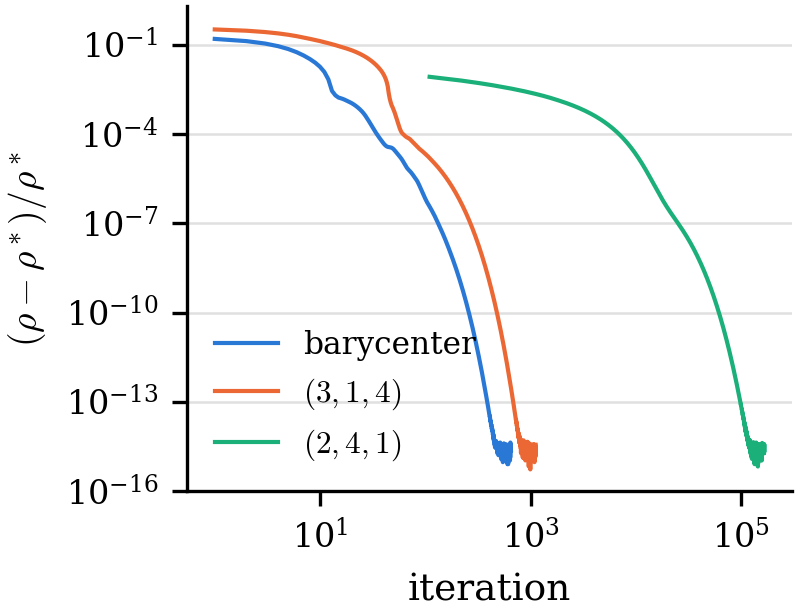
\includegraphics[width=0.4\textwidth]{fig_yogi_conv_excess}}\hspace{0.1\textwidth}
\subfloat[stationarity measure]{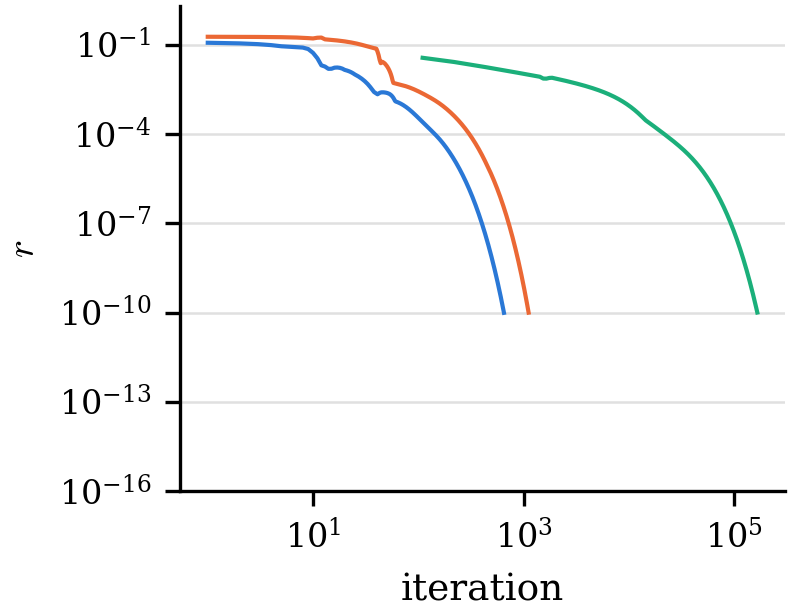
\includegraphics[width=0.4\textwidth]{fig_yogi_conv_r}}
\caption{Projected Yogi on the weekly instance from three starts.}\label{t-fig-conv}
\end{figure}

% \paragraph{Thirty-six instances.} To test whether the barycenter is a reliable
% start we varied the data in $36$ instances: the first-dose budget $b_{1i}$
\paragraph{Thirty-six instances.} We ran projected Yogi from the barycenter
on $36$ instances with varied data: the first-dose budget $b_{1i}$
weekly or daily ($b_{1i}/7$); the ratios
\begin{equation}
\frac{(b_{2i},b_{3i})}{b_{1i}}\in\left\{\left(\tfrac1{16},\tfrac1{16}\right),\left(\tfrac14,\tfrac14\right),(1,1),(4,4),\left(\tfrac12,\tfrac18\right),\left(\tfrac18,\tfrac12\right)\right\};
\end{equation}
and $\sigma_{2,ij}$, $\sigma_{3,ij}$ equal to $P_{ij}$, or equal to
$P_{ij}e^{Z_{ij}/2}$ and $P_{ij}e^{Z'_{ij}/2}$ with independent standard
normal $Z$, $Z'$, for two seeds. Seed $s\in\{1,2\}$ means that $Z$ and then
$Z'$, each $m\times n$ with the entries in row order, are drawn by
\texttt{numpy.random.default\_rng(s).standard\_normal}.
% For each instance $\rho_{\mathrm{best}}$ is
% the smallest value known: that of $69$ runs of the trust region interior point
% method of~\cite{1999Byrd_Hribar_Nocedal} in all $3N$ variables, from the $49$
% starts above and $20$ random points of $\mathcal{S}$, or that of
% projected Yogi from the barycenter if it is smaller. A run is
% successful if its $\rho$ is at most $(1+10^{-7})\rho_{\mathrm{best}}$.

From the barycenter, projected Yogi takes between $545$ and
$10897$ iterations, $66$~s for all $36$ instances, and ends with $r<10^{-10}$
in every instance.
% It is successful in $31$ instances, $14$ of the $18$
% weekly and $17$ of the $18$ daily. In two of them its value is smaller than
% that of all $69$ interior point runs, by $0.13$ and $0.025$ per cent, and is
% $\rho_{\mathrm{best}}$. Table~\ref{t-tab-yogi-inst} lists these two (top) and
% the five instances in which it is not successful (bottom), with the best $\rho$
% of the interior point runs, $\rho$ of projected Yogi, and its relative excess
% $(\rho-\rho_{\mathrm{best}})/\rho_{\mathrm{best}}$. Four of the five are weekly,
% two of them with the smallest budgets $b_{2i}=b_{3i}=b_{1i}/16$; the misses are
% up to $1.2$ per cent. At these five endpoints $r<10^{-10}$, so they are points
% satisfying the Karush--Kuhn--Tucker conditions to this accuracy with $\rho$
% above $\rho_{\mathrm{best}}$, and $\Theta$ is not convex on these instances.

\begin{remark}\label{t-rem-interior}
For comparison, on each of the $36$ instances we also ran the trust region
interior point method of~\cite{1999Byrd_Hribar_Nocedal} in all $3N$
variables, $69$ times: from the $49$ starts above and from $20$ random points
of $\mathcal{S}$. Let $\rho_{\mathrm{best}}$ be the smallest value given by
these runs and by projected Yogi from the barycenter. In $31$ of the $36$
instances projected Yogi from the barycenter gives $\rho$ at most
$(1+10^{-7})\rho_{\mathrm{best}}$, and in two of these its value is smaller
than that of all $69$ interior point runs, by $0.13$ and $0.025$ per cent. In
the other five, four of them weekly, its $\rho$ exceeds $\rho_{\mathrm{best}}$
by up to $1.2$ per cent, while $r<10^{-10}$ at its endpoint. These endpoints
satisfy the Karush--Kuhn--Tucker conditions to this accuracy with $\rho$ above
$\rho_{\mathrm{best}}$, so $\Theta$ is not convex on these instances, and a
single start does not in general give the global minimum.
\end{remark}
%
% \begin{table}[ht]
% \centering
% \small
% \begin{tabular}{lllccc}
% \hline
% budget & $(b_{2i},b_{3i})/b_{1i}$ & $\sigma_2,\sigma_3$ & interior point &
% projected Yogi & relative excess\\
% \hline
% weekly & $(\tfrac14,\tfrac14)$       & seed $2$ & $1.7118$ & $1.7095$ & $0$\\
% weekly & $(\tfrac18,\tfrac12)$       & $P$      & $1.3088$ & $1.3085$ & $0$\\
% \hline
% weekly & $(\tfrac1{16},\tfrac1{16})$ & $P$      & $2.5032$ & $2.5335$ & $1.2\cdot 10^{-2}$\\
% weekly & $(\tfrac1{16},\tfrac1{16})$ & seed $2$ & $2.4253$ & $2.4384$ & $5.4\cdot 10^{-3}$\\
% weekly & $(\tfrac18,\tfrac12)$       & seed $1$ & $1.2363$ & $1.2376$ & $1.1\cdot 10^{-3}$\\
% weekly & $(\tfrac18,\tfrac12)$       & seed $2$ & $1.3770$ & $1.3820$ & $3.6\cdot 10^{-3}$\\
% daily  & $(\tfrac1{16},\tfrac1{16})$ & $P$      & $4.0391$ & $4.0403$ & $2.9\cdot 10^{-4}$\\
% \hline
% \end{tabular}
% \caption{Projected Yogi from the barycenter: the instances in which it
% improves on the interior point runs, and those in which it is not
% successful.}\label{t-tab-yogi-inst}
% \end{table}

Figure~\ref{t-fig-alloc-yogi} shows, for two of the
weekly instances, the allocations $\chi_{k,ij}$ at the endpoint of projected
Yogi from the barycenter, in units of $10^{-3}$ per day, one line per
location. The first instance has $b_{2i}=b_{3i}=b_{1i}/4$ and $\sigma_2$,
$\sigma_3$ of seed $2$, and $\rho=1.7095$; the second $b_{2i}=b_{1i}/8$,
$b_{3i}=b_{1i}/2$ and $\sigma_2=\sigma_3=P$, and $\rho=1.3085$. In the first
instance the group $60+$ of the South receives no second or third doses, and
their budget goes to the groups $0$--$59$ of the South; in the second the same
holds for the group $60+$ of the West. As for the single dose, where the group
$60+$ receives no doses at the minimizer, doses go away from this group.

% Figures~\ref{t-fig-alloc-s2-k1}--\ref{t-fig-alloc-s2-k3}
% and~\ref{t-fig-alloc-p-k1}--\ref{t-fig-alloc-p-k3} show, for the two
% instances at the top of Table~\ref{t-tab-yogi-inst}, the allocations
% $\chi_{k,ij}$ at the endpoint of projected Yogi and at that of the
% interior point method from the barycenter, which gives the best of the $69$
% interior point values: one figure per dose type, in units of $10^{-3}$ per
% day, the interior point endpoint on the left and projected Yogi on the right,
% one line per location and the same scale in both plots. The first instance has
% $b_{2i}=b_{3i}=b_{1i}/4$ and $\sigma_2$, $\sigma_3$ of seed $2$; the second
% $b_{2i}=b_{1i}/8$, $b_{3i}=b_{1i}/2$ and $\sigma_2=\sigma_3=P$. The two allocations differ mainly in one location. In
% the first instance the interior point endpoint gives the group $60+$ of the
% South $\chi_{2}=0.0162$ and $\chi_{3}=0.0211$ per day, and that of
% projected Yogi gives this group no second or third doses and their
% budget to the groups $0$--$59$ of the South. In the second instance the same
% holds for the group $60+$ of the West, with $\chi_{2}=0.0098$ and
% $\chi_{3}=0.0181$ per day at the interior point endpoint. In the other three
% locations the entries above $10^{-3}$ per day agree to $2.2$ per cent; the
% smaller ones, first doses to the group $60+$, differ by up to
% $3\cdot 10^{-4}$ per day. As for the single dose, where the group $60+$
% receives no doses at the minimizer, the smaller value moves doses away from
% this group.

\begin{figure}[htbp]
\centering
\subfloat[$\chi_1$, first instance]{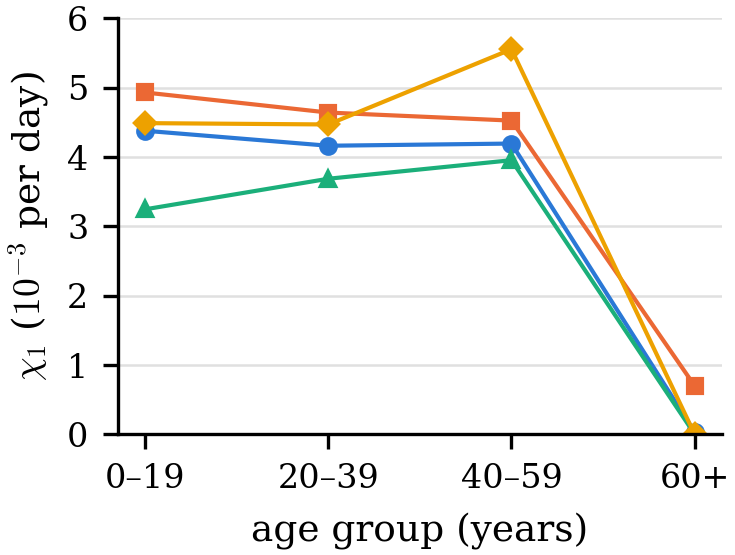
\includegraphics[width=0.32\textwidth]{fig_alloc_s2_yogi_k1}}\hfill
\subfloat[$\chi_2$, first instance]{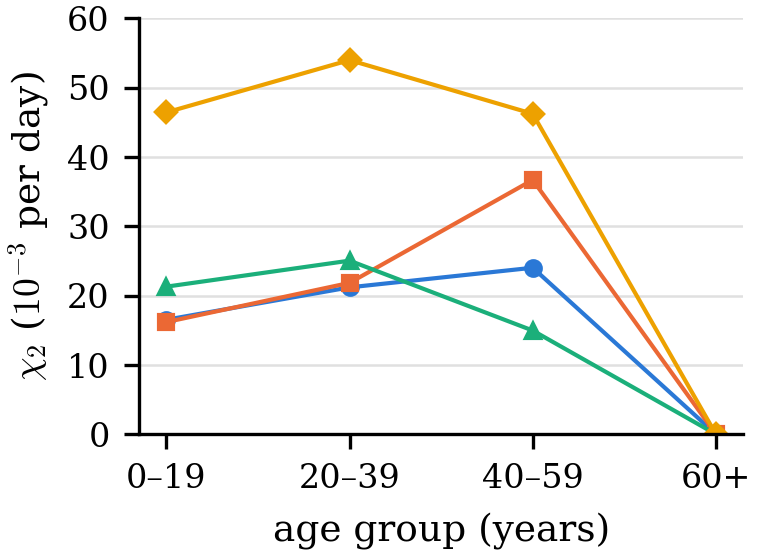
\includegraphics[width=0.32\textwidth]{fig_alloc_s2_yogi_k2}}\hfill
\subfloat[$\chi_3$, first instance]{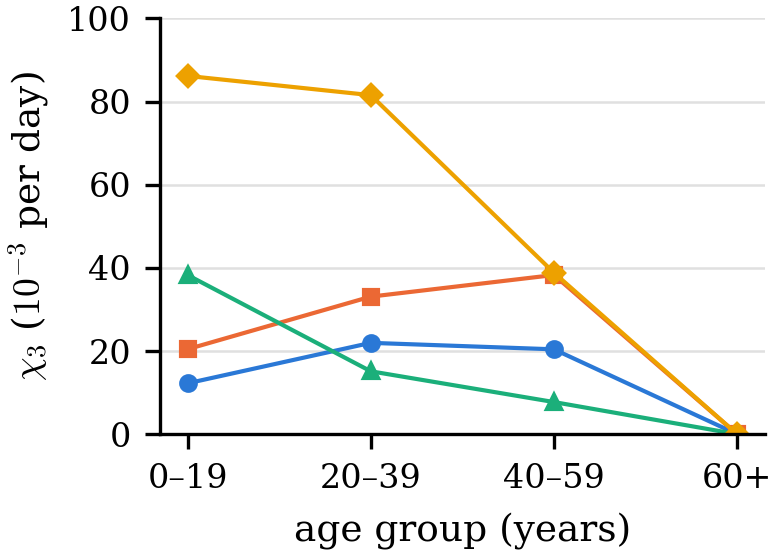
\includegraphics[width=0.32\textwidth]{fig_alloc_s2_yogi_k3}}\\
\subfloat[$\chi_1$, second instance]{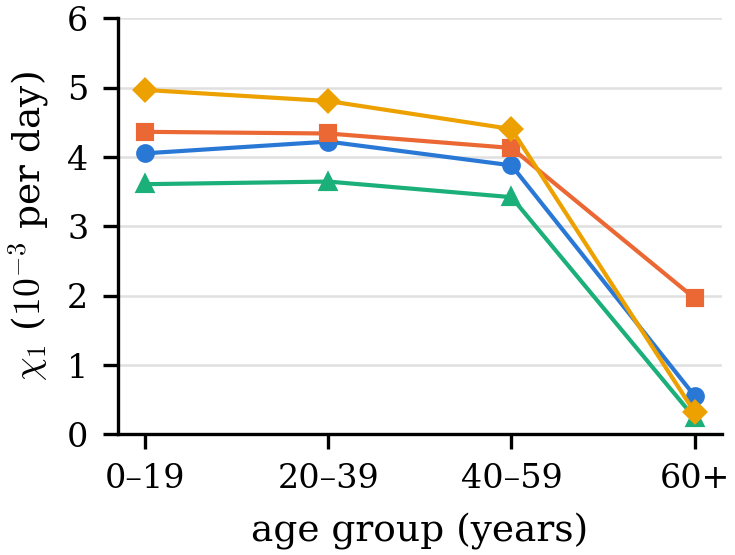
\includegraphics[width=0.32\textwidth]{fig_alloc_p_yogi_k1}}\hfill
\subfloat[$\chi_2$, second instance]{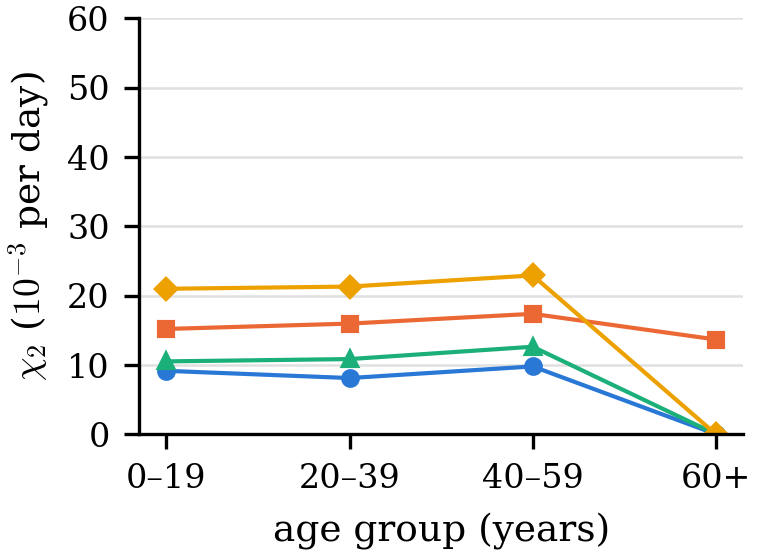
\includegraphics[width=0.32\textwidth]{fig_alloc_p_yogi_k2}}\hfill
\subfloat[$\chi_3$, second instance]{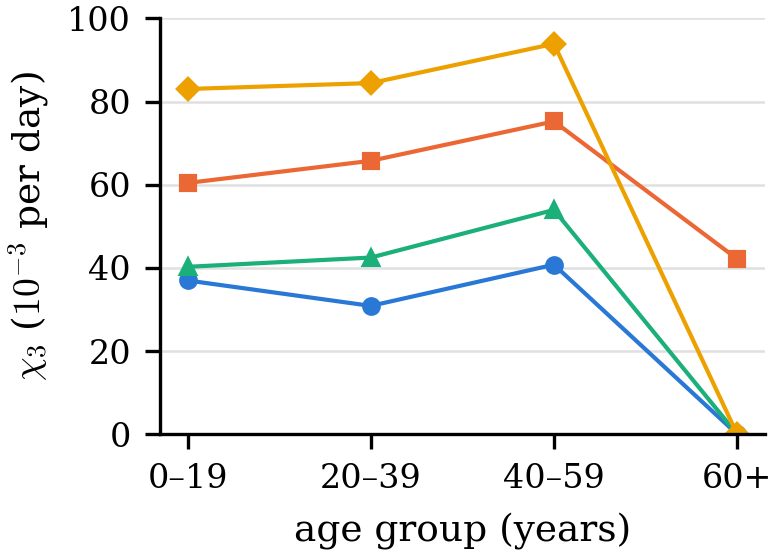
\includegraphics[width=0.32\textwidth]{fig_alloc_p_yogi_k3}}
\caption{The allocations at the endpoint of projected Yogi for the weekly
budget. Top row: $b_{2i}=b_{3i}=b_{1i}/4$, $\sigma_2$, $\sigma_3$ of seed $2$,
$\rho=1.7095$. Bottom row: $b_{2i}=b_{1i}/8$, $b_{3i}=b_{1i}/2$,
$\sigma_2=\sigma_3=P$, $\rho=1.3085$.}\label{t-fig-alloc-yogi}
\end{figure}

% \begin{figure}[htbp]
% \centering
% \subfloat[$\chi_1$]{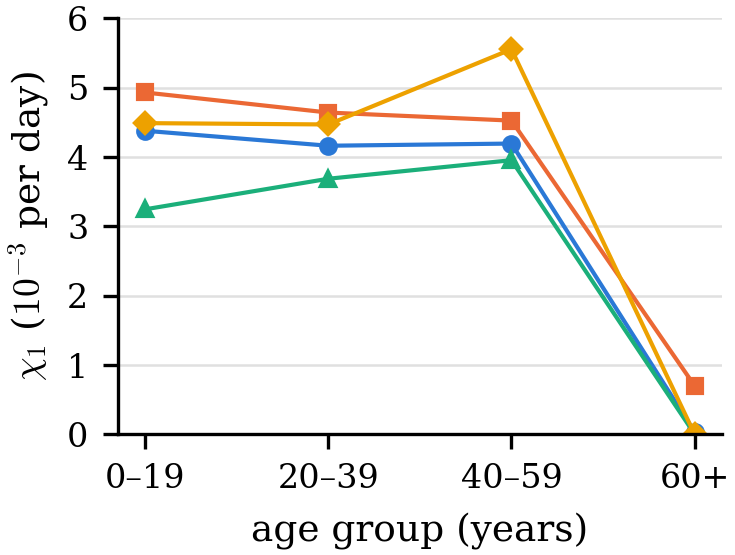
\includegraphics[width=0.4\textwidth]{fig_alloc_s2_yogi_k1}}\hspace{0.1\textwidth}
% \subfloat[$\chi_2$]{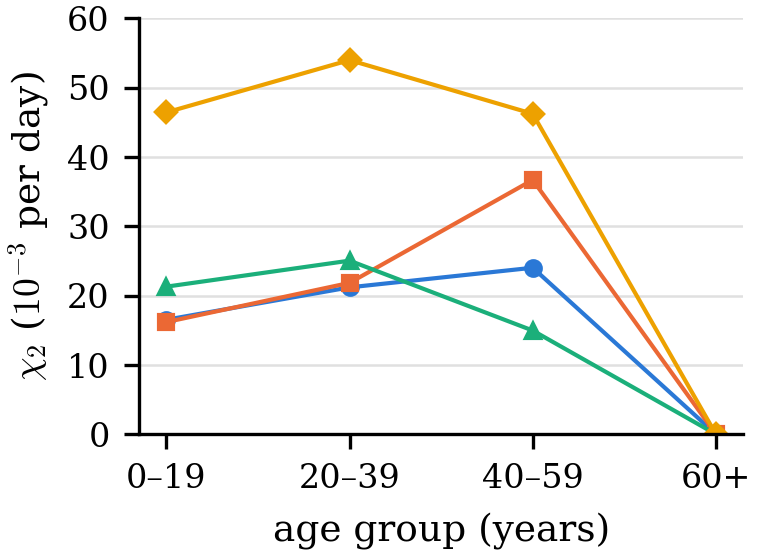
\includegraphics[width=0.4\textwidth]{fig_alloc_s2_yogi_k2}}\\
% \subfloat[$\chi_3$]{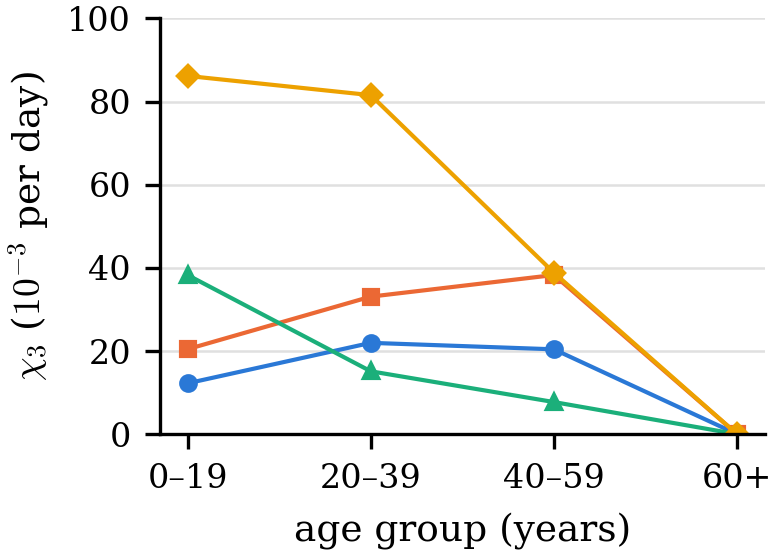
\includegraphics[width=0.4\textwidth]{fig_alloc_s2_yogi_k3}}
% \caption{The allocations at the endpoint of projected Yogi, $\rho=1.7095$,
% for the weekly budget, $b_{2i}=b_{3i}=b_{1i}/4$, and $\sigma_2$, $\sigma_3$
% of seed $2$.}\label{t-fig-alloc-s2}
% \end{figure}
%
% \begin{figure}[htbp]
% \centering
% \subfloat[$\chi_1$]{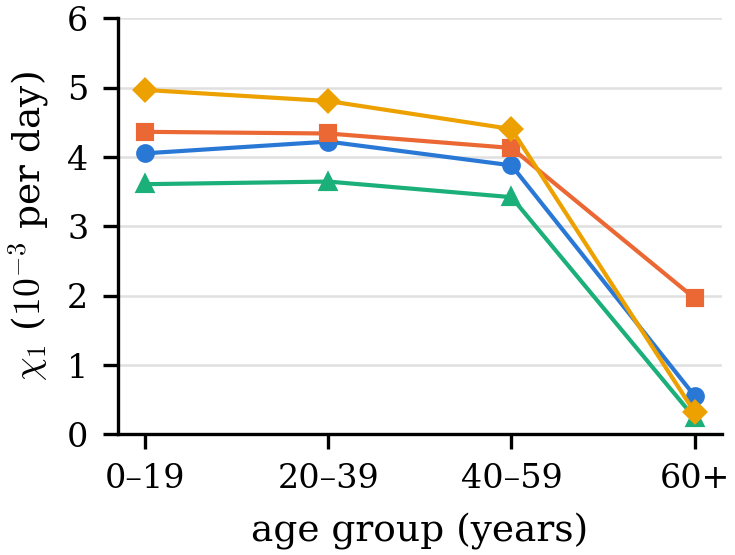
\includegraphics[width=0.4\textwidth]{fig_alloc_p_yogi_k1}}\hspace{0.1\textwidth}
% \subfloat[$\chi_2$]{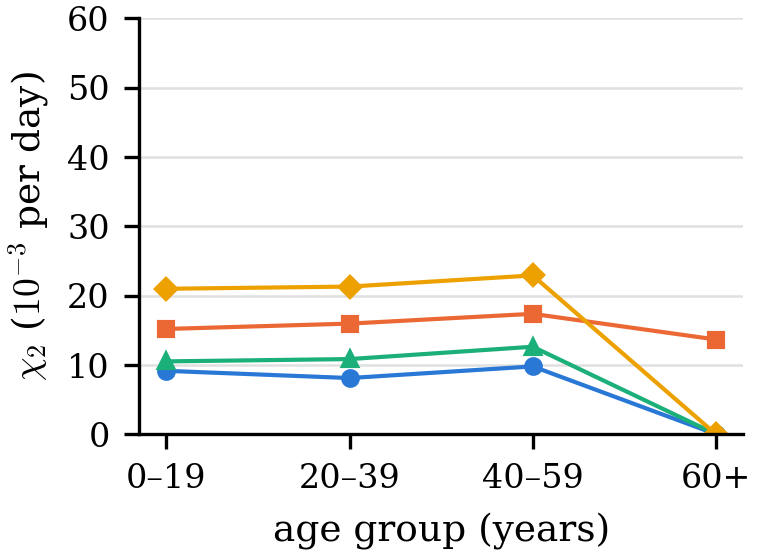
\includegraphics[width=0.4\textwidth]{fig_alloc_p_yogi_k2}}\\
% \subfloat[$\chi_3$]{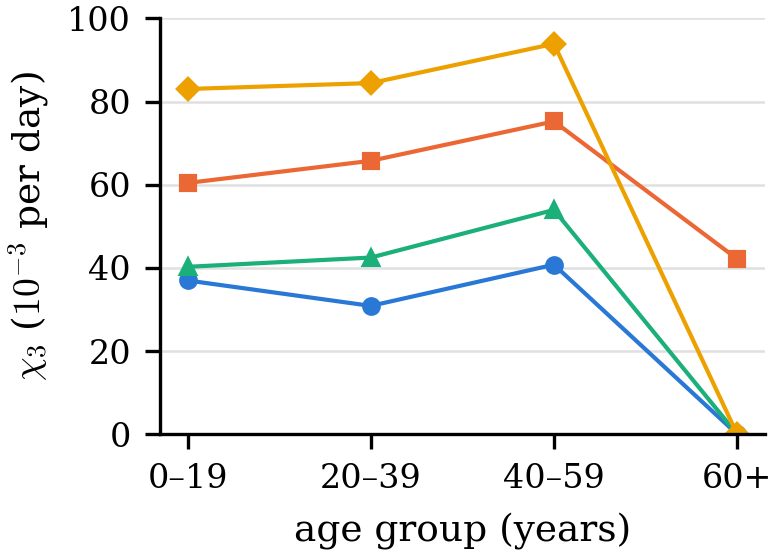
\includegraphics[width=0.4\textwidth]{fig_alloc_p_yogi_k3}}
% \caption{The allocations at the endpoint of projected Yogi, $\rho=1.3085$,
% for the weekly budget, $b_{2i}=b_{1i}/8$, $b_{3i}=b_{1i}/2$, and
% $\sigma_2=\sigma_3=P$.}\label{t-fig-alloc-p}
% \end{figure}

% \begin{figure}[htbp]
% \centering
% \subfloat[interior point method, $\rho=1.7118$]{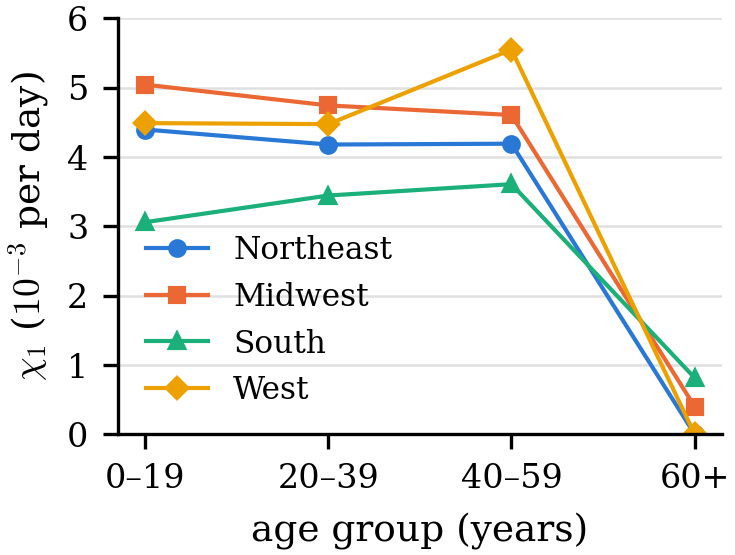
\includegraphics[width=0.4\textwidth]{fig_alloc_s2_joint_k1}}\hspace{0.1\textwidth}
% \subfloat[projected Yogi, $\rho=1.7095$]{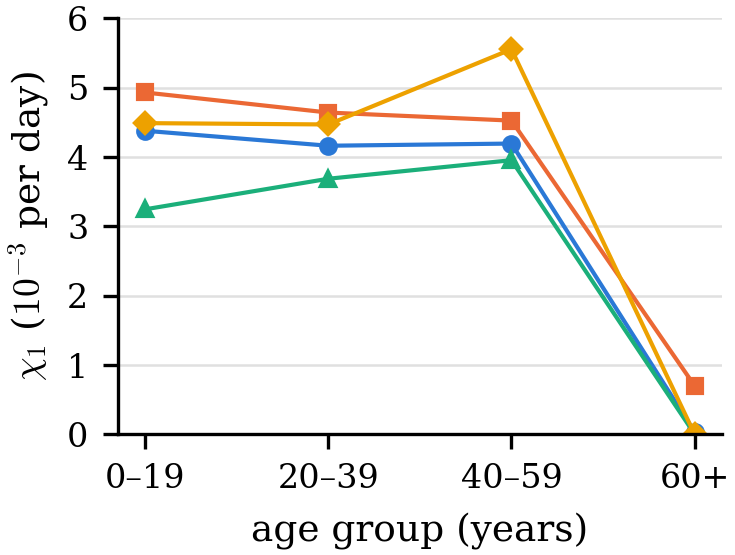
\includegraphics[width=0.4\textwidth]{fig_alloc_s2_yogi_k1}}
% \caption{The allocation $\chi_1$ for the weekly budget,
% $b_{2i}=b_{3i}=b_{1i}/4$, and $\sigma_2$, $\sigma_3$ of seed $2$.}\label{t-fig-alloc-s2-k1}
% \end{figure}
%
% \begin{figure}[htbp]
% \centering
% \subfloat[interior point method, $\rho=1.7118$]{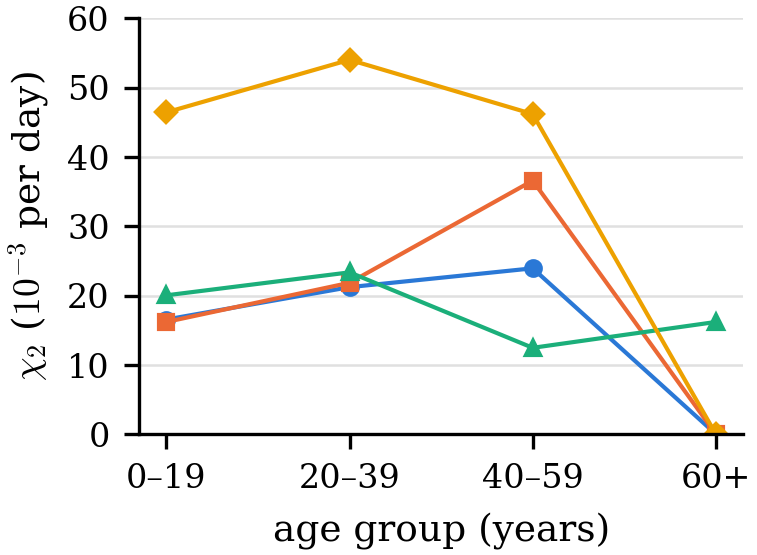
\includegraphics[width=0.4\textwidth]{fig_alloc_s2_joint_k2}}\hspace{0.1\textwidth}
% \subfloat[projected Yogi, $\rho=1.7095$]{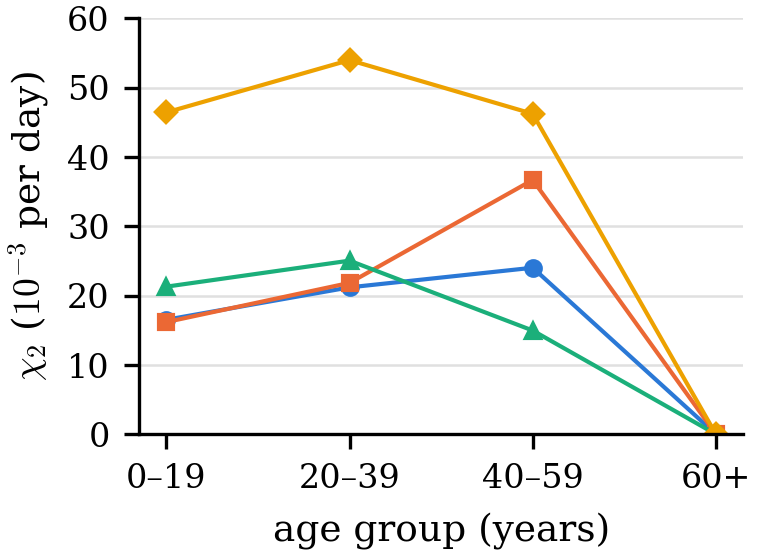
\includegraphics[width=0.4\textwidth]{fig_alloc_s2_yogi_k2}}
% \caption{The allocation $\chi_2$ for the weekly budget,
% $b_{2i}=b_{3i}=b_{1i}/4$, and $\sigma_2$, $\sigma_3$ of seed $2$.}\label{t-fig-alloc-s2-k2}
% \end{figure}
%
% \begin{figure}[htbp]
% \centering
% \subfloat[interior point method, $\rho=1.7118$]{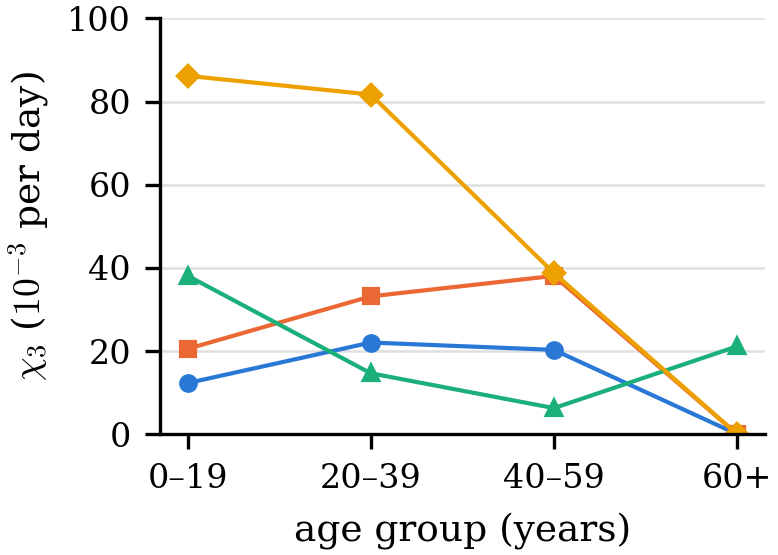
\includegraphics[width=0.4\textwidth]{fig_alloc_s2_joint_k3}}\hspace{0.1\textwidth}
% \subfloat[projected Yogi, $\rho=1.7095$]{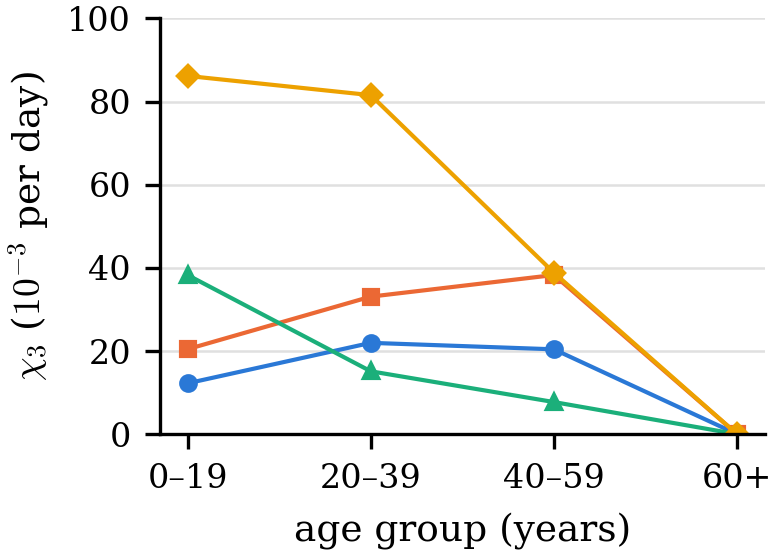
\includegraphics[width=0.4\textwidth]{fig_alloc_s2_yogi_k3}}
% \caption{The allocation $\chi_3$ for the weekly budget,
% $b_{2i}=b_{3i}=b_{1i}/4$, and $\sigma_2$, $\sigma_3$ of seed $2$.}\label{t-fig-alloc-s2-k3}
% \end{figure}
%
% \begin{figure}[htbp]
% \centering
% \subfloat[interior point method, $\rho=1.3088$]{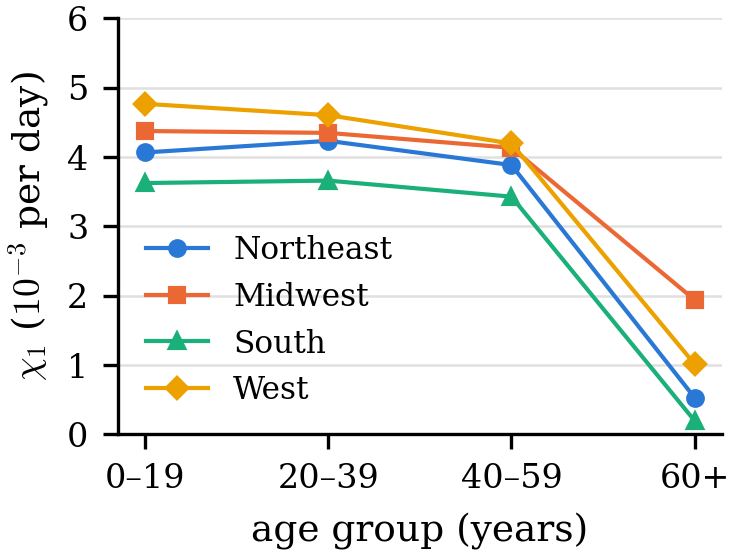
\includegraphics[width=0.4\textwidth]{fig_alloc_p_joint_k1}}\hspace{0.1\textwidth}
% \subfloat[projected Yogi, $\rho=1.3085$]{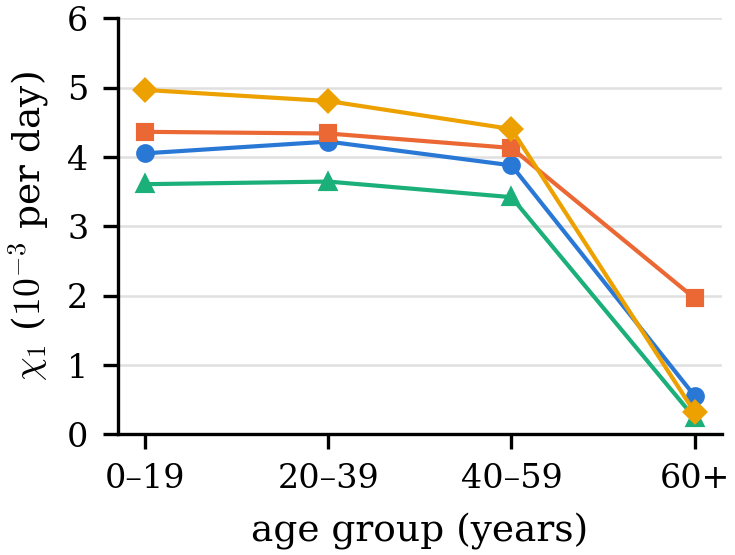
\includegraphics[width=0.4\textwidth]{fig_alloc_p_yogi_k1}}
% \caption{The allocation $\chi_1$ for the weekly budget,
% $b_{2i}=b_{1i}/8$, $b_{3i}=b_{1i}/2$, and $\sigma_2=\sigma_3=P$.}\label{t-fig-alloc-p-k1}
% \end{figure}
%
% \begin{figure}[htbp]
% \centering
% \subfloat[interior point method, $\rho=1.3088$]{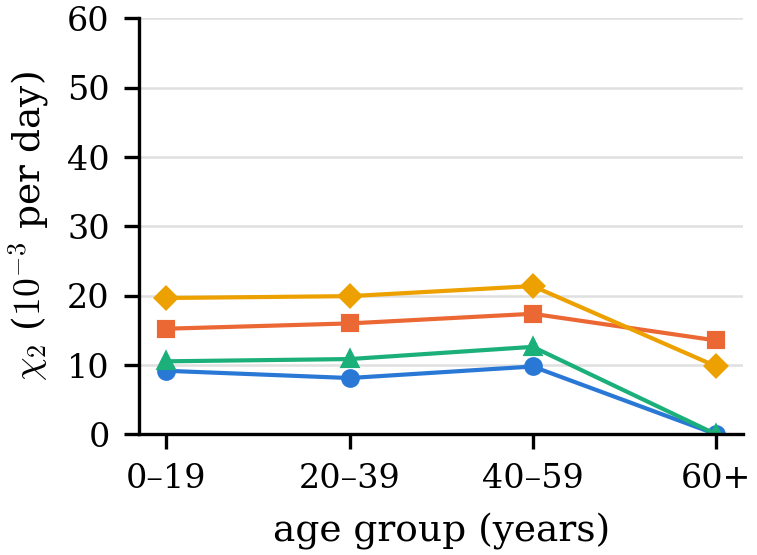
\includegraphics[width=0.4\textwidth]{fig_alloc_p_joint_k2}}\hspace{0.1\textwidth}
% \subfloat[projected Yogi, $\rho=1.3085$]{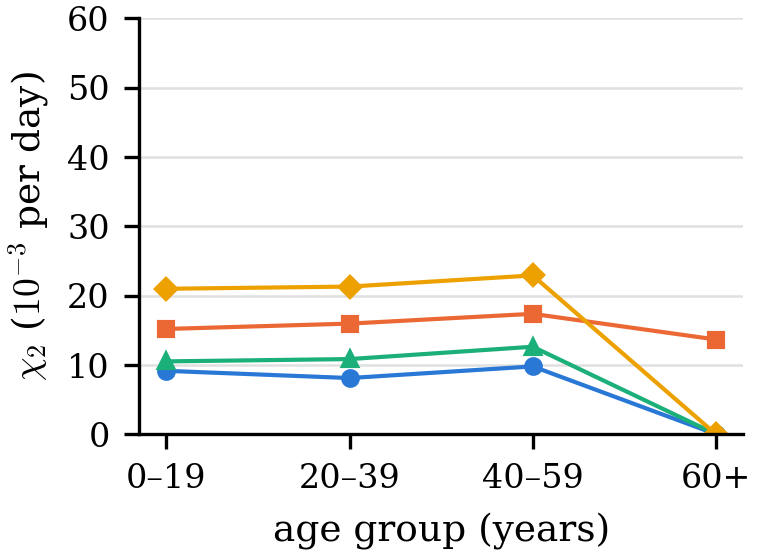
\includegraphics[width=0.4\textwidth]{fig_alloc_p_yogi_k2}}
% \caption{The allocation $\chi_2$ for the weekly budget,
% $b_{2i}=b_{1i}/8$, $b_{3i}=b_{1i}/2$, and $\sigma_2=\sigma_3=P$.}\label{t-fig-alloc-p-k2}
% \end{figure}
%
% \begin{figure}[htbp]
% \centering
% \subfloat[interior point method, $\rho=1.3088$]{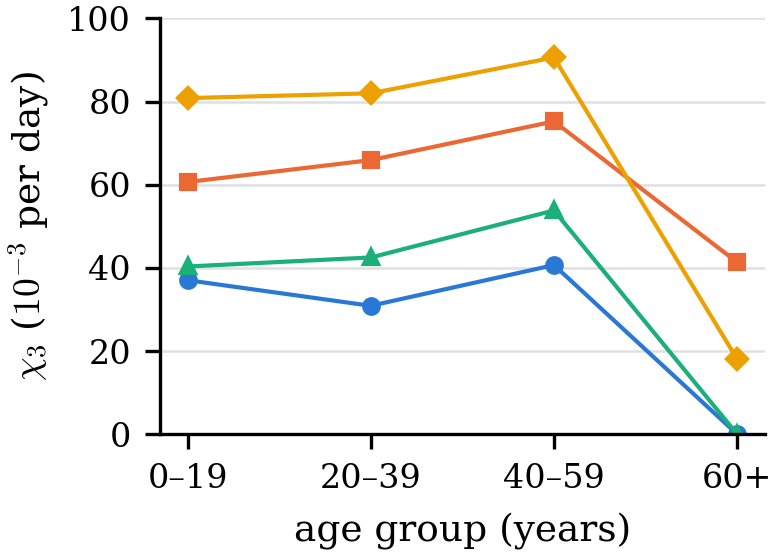
\includegraphics[width=0.4\textwidth]{fig_alloc_p_joint_k3}}\hspace{0.1\textwidth}
% \subfloat[projected Yogi, $\rho=1.3085$]{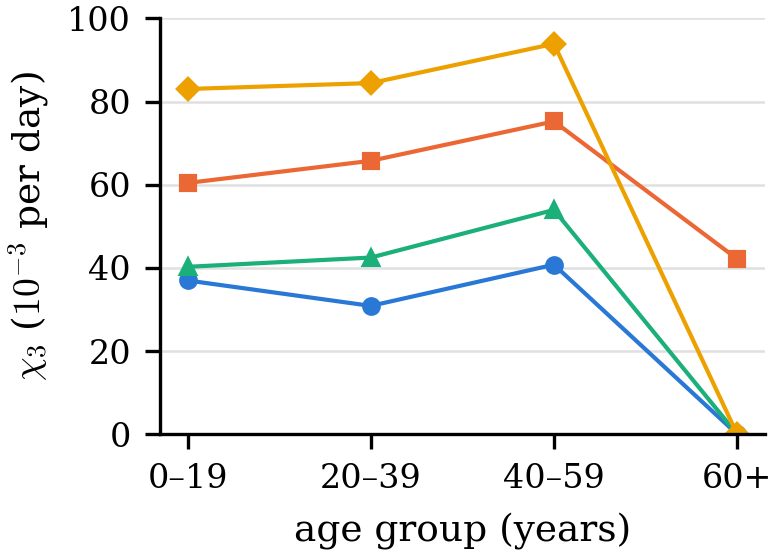
\includegraphics[width=0.4\textwidth]{fig_alloc_p_yogi_k3}}
% \caption{The allocation $\chi_3$ for the weekly budget,
% $b_{2i}=b_{1i}/8$, $b_{3i}=b_{1i}/2$, and $\sigma_2=\sigma_3=P$.}\label{t-fig-alloc-p-k3}
% \end{figure}

In practice the method should be run from several starts, the barycenter, the
starts near the vertices and random points, and the smallest value kept; no
single start is guaranteed to give the global minimum. These tests use second
and third dose data chosen for lack of data, $\sigma_2$ and $\sigma_3$ built
from the numbers of partially protected individuals.

The computations are in the following python files:
\begin{itemize}
\item \texttt{check\_block2.py}: the sampling for the second dose in
Section~\ref{M-sec-three};
\item \texttt{yogi\_three\_dose.py}: projected Yogi on the weekly
instance from the $49$ starts, and Table~\ref{t-tab-yogi};
% \item \texttt{yogi\_instances\_three\_dose.py}: the $36$ instances, and
% Table~\ref{t-tab-yogi-inst};
% \item \texttt{test\_barycenter\_three\_dose.py}: the $69$ interior point runs
% per instance;
\item \texttt{yogi\_instances\_three\_dose.py}: the $36$ instances;
\item \texttt{test\_barycenter\_three\_dose.py}: the $69$ interior point runs
per instance in Remark~\ref{t-rem-interior};
\item \texttt{plot\_yogi\_three\_dose.py}: the data of
Figures~\ref{t-fig-conv} and~\ref{t-fig-alloc-yogi}.
% Figures~\ref{t-fig-conv} and~\ref{t-fig-alloc-s2-k1}--\ref{t-fig-alloc-p-k3}.
\end{itemize}

\bibliographystyle{plain}
\bibliography{../bib_mb}

\end{document}
